\documentclass[a4paper,landscape]{article}
\usepackage{tikz}
\usepackage{gensymb}
\usepackage[utf8]{inputenc}
\usepackage[left=1cm,top=1cm,right=1cm,bottom=1cm,verbose,nohead,nofoot]{geometry}
\usepackage{fix-cm}
\begin{document}
\pagenumbering{gobble}\newcommand\HUGE{\fontsize{100}{120}\selectfont}
\thispagestyle{empty}
\begin{center} 
\large\textbf{1\degree Andar}\\
\vspace*{5px} 
\large
\textmd{Comprimento: 100  -  Profundidade: 100  -  Altura: 30 (cm)}\\ \end{center}
\centering
\resizebox{!}{0.9\textheight}{%
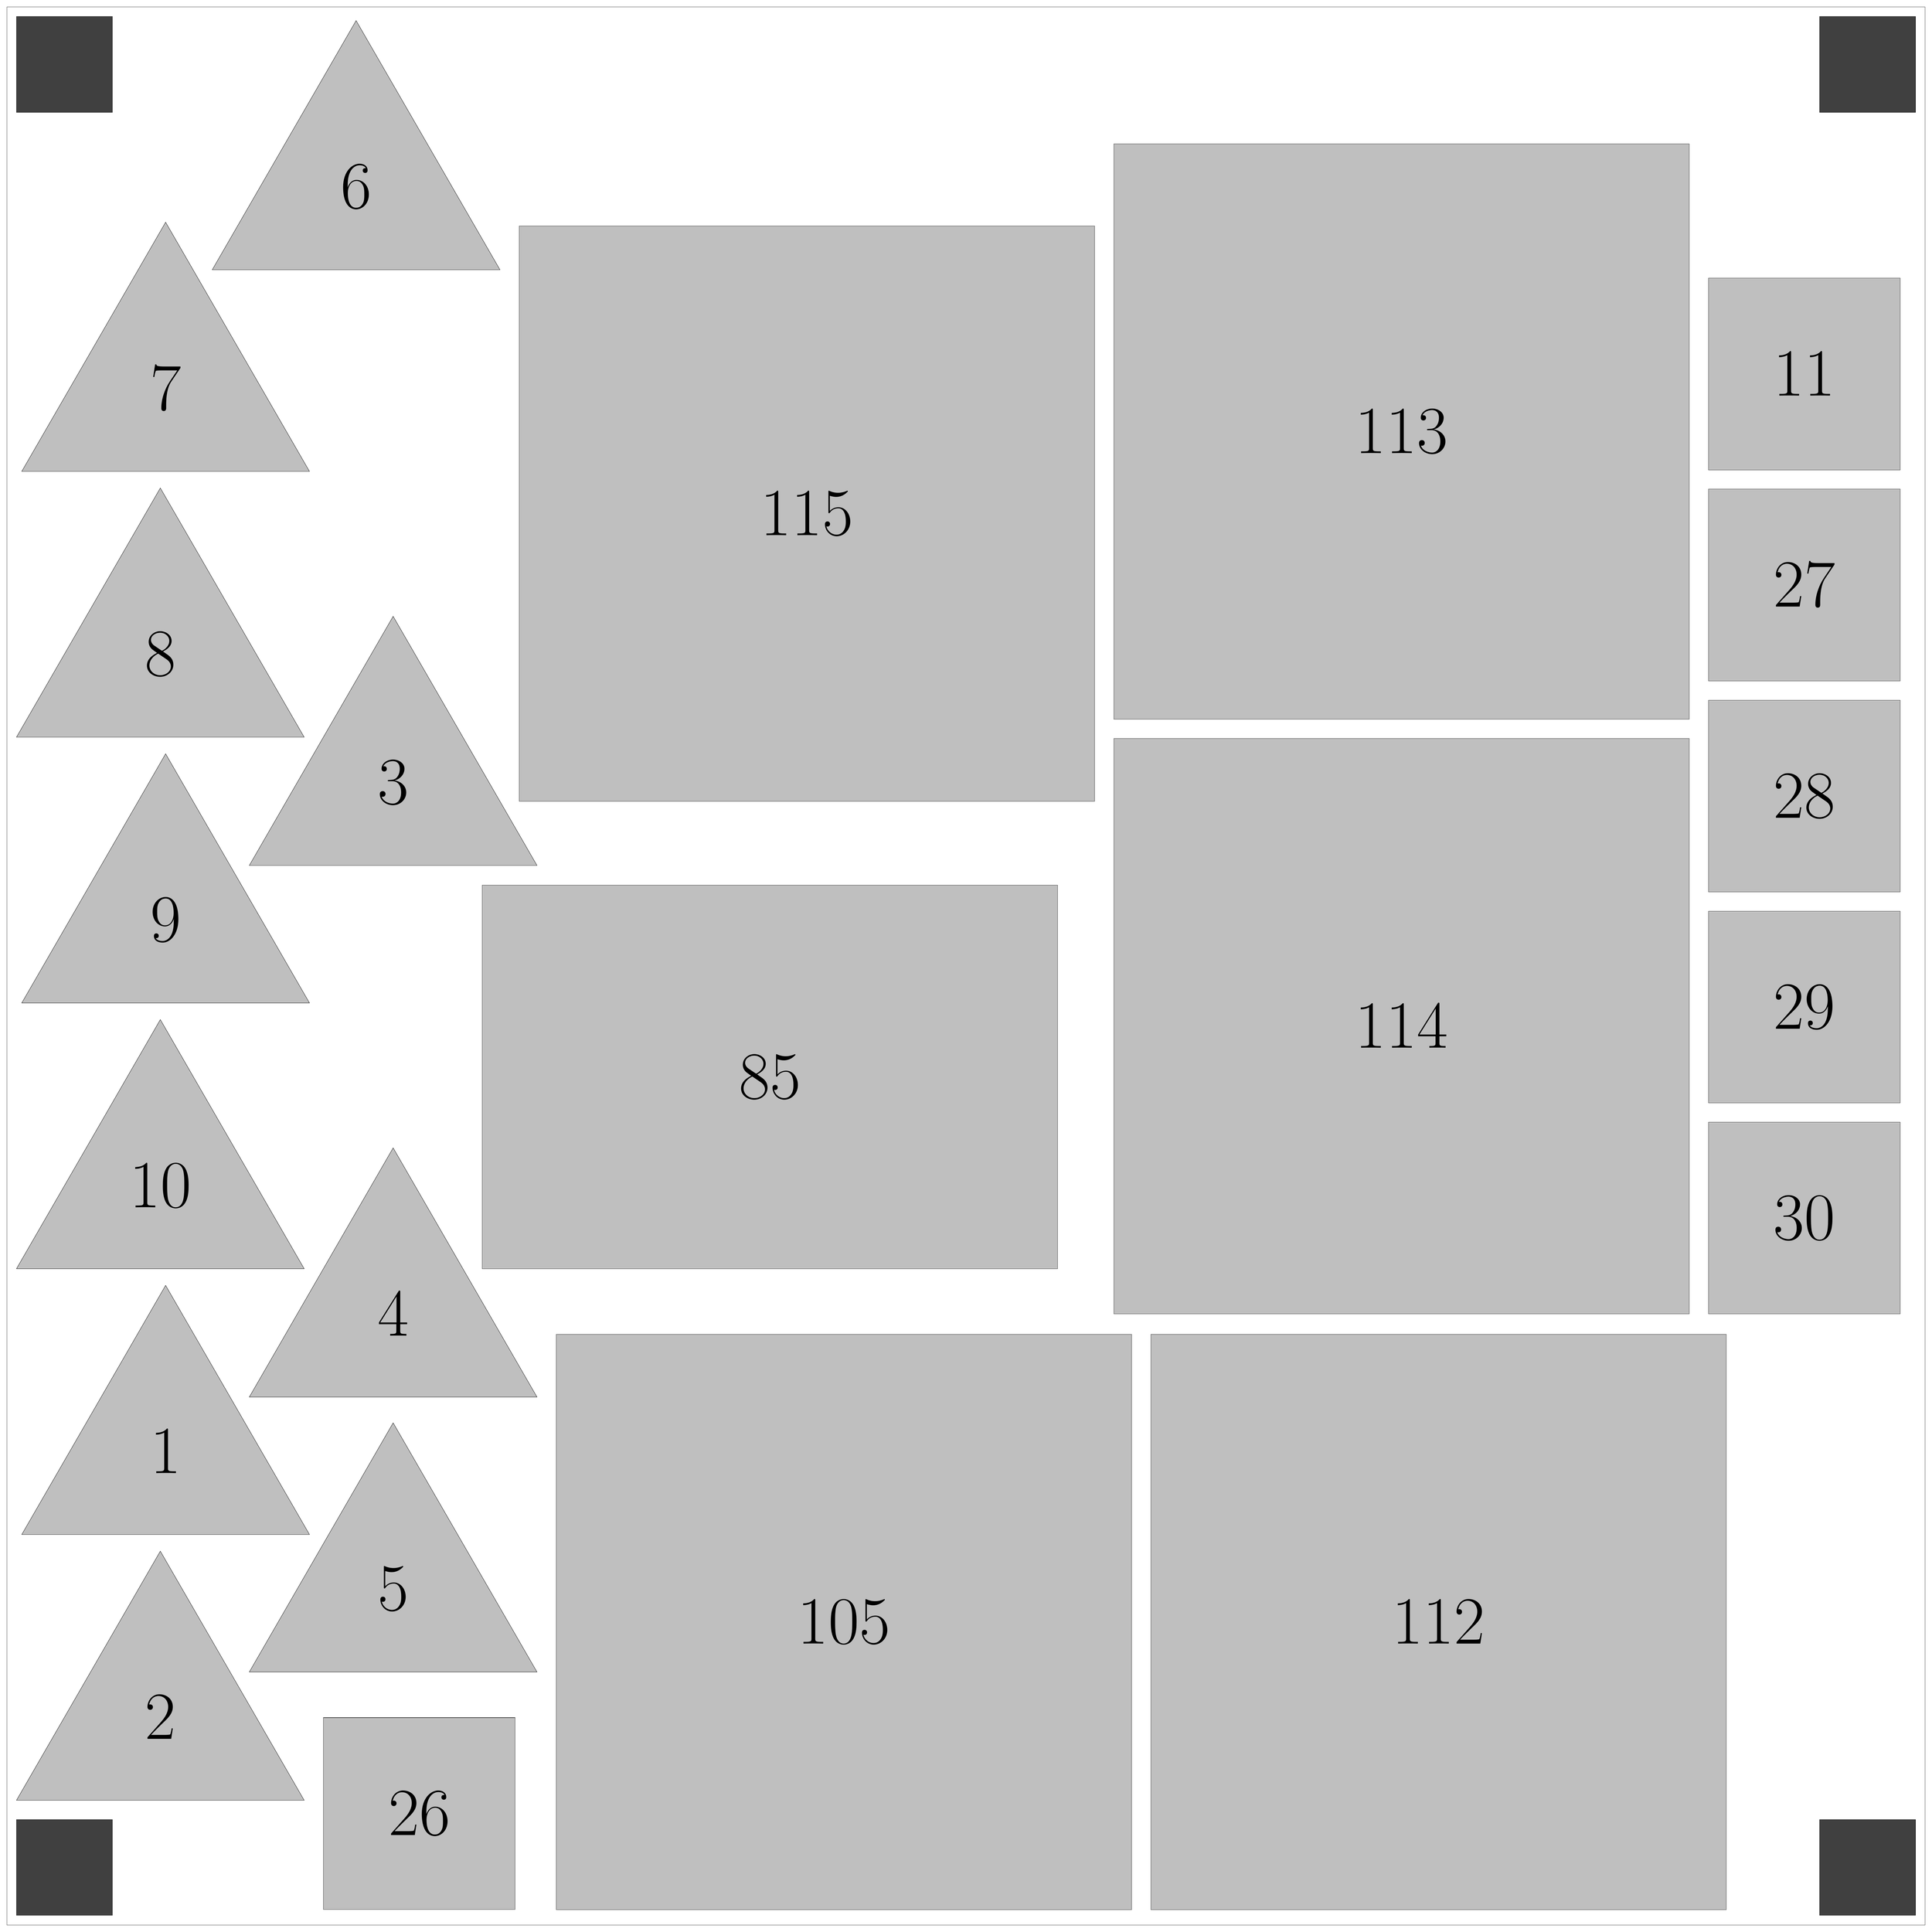
\begin{tikzpicture}\draw[black] (0,0) rectangle (100, 100);
\draw[black, fill=darkgray] (0.5,0.5) rectangle (5.5, 5.5);
\draw[black, fill=darkgray] (0.5,94.5) rectangle (5.5, 99.5);
\draw[black, fill=darkgray] (94.5,0.5) rectangle (99.5, 5.5);
\draw[black, fill=darkgray] (94.5,94.5) rectangle (99.5, 99.5);
\draw[black, fill=lightgray] (0.5,6.5) -- (15.5, 6.5) -- (8, 19.4904) -- cycle;
\draw (8, 10.8301) node {\fontsize{100}{120}\selectfont 2};
\draw[black, fill=lightgray] (0.775862,20.3564) -- (15.7759, 20.3564) -- (8.27586, 33.3468) -- cycle;
\draw (8.27586, 24.6865) node {\fontsize{100}{120}\selectfont 1};
\draw[black, fill=lightgray] (0.5,34.2128) -- (15.5, 34.2128) -- (8, 47.2032) -- cycle;
\draw (8, 38.5429) node {\fontsize{100}{120}\selectfont 10};
\draw[black, fill=lightgray] (0.775862,48.0692) -- (15.7759, 48.0692) -- (8.27586, 61.0596) -- cycle;
\draw (8.27586, 52.3993) node {\fontsize{100}{120}\selectfont 9};
\draw[black, fill=lightgray] (0.5,61.9256) -- (15.5, 61.9256) -- (8, 74.916) -- cycle;
\draw (8, 66.2558) node {\fontsize{100}{120}\selectfont 8};
\draw[black, fill=lightgray] (0.775862,75.782) -- (15.7759, 75.782) -- (8.27586, 88.7724) -- cycle;
\draw (8.27586, 80.1122) node {\fontsize{100}{120}\selectfont 7};
\draw[black, fill=lightgray] (10.7069,86.2938) -- (25.7069, 86.2938) -- (18.2069, 99.2842) -- cycle;
\draw (18.2069, 90.6239) node {\fontsize{100}{120}\selectfont 6};
\draw[black, fill=lightgray] (12.6379,13.1893) -- (27.6379, 13.1893) -- (20.1379, 26.1797) -- cycle;
\draw (20.1379, 17.5194) node {\fontsize{100}{120}\selectfont 5};
\draw[black, fill=lightgray] (12.6379,27.5235) -- (27.6379, 27.5235) -- (20.1379, 40.5139) -- cycle;
\draw (20.1379, 31.8536) node {\fontsize{100}{120}\selectfont 4};
\draw[black, fill=lightgray] (12.6379,55.2363) -- (27.6379, 55.2363) -- (20.1379, 68.2267) -- cycle;
\draw (20.1379, 59.5665) node {\fontsize{100}{120}\selectfont 3};
\draw[black, fill=lightgray] (26.7069,58.581) rectangle (56.7069, 88.581);
\draw (41.7069, 73.581) node {\fontsize{100}{120}\selectfont 115};
\draw[black, fill=lightgray] (28.6379,0.799375) rectangle (58.6379, 30.7994);
\draw (43.6379, 15.7994) node {\fontsize{100}{120}\selectfont 105};
\draw[black, fill=lightgray] (57.7069,31.8568) rectangle (87.7069, 61.8568);
\draw (72.7069, 46.8568) node {\fontsize{100}{120}\selectfont 114};
\draw[black, fill=lightgray] (57.7069,62.8568) rectangle (87.7069, 92.8568);
\draw (72.7069, 77.8568) node {\fontsize{100}{120}\selectfont 113};
\draw[black, fill=lightgray] (59.6379,0.799375) rectangle (89.6379, 30.7994);
\draw (74.6379, 15.7994) node {\fontsize{100}{120}\selectfont 112};
\draw[black, fill=lightgray] (24.7759,34.2128) rectangle (54.7759, 54.2128);
\draw (39.7759, 44.2128) node {\fontsize{100}{120}\selectfont 85};
\draw[black, fill=lightgray] (16.5,0.810345) rectangle (26.5, 10.8103);
\draw (21.5, 5.81034) node {\fontsize{100}{120}\selectfont 26};
\draw[black, fill=lightgray] (88.7069,31.8568) rectangle (98.7069, 41.8568);
\draw (93.7069, 36.8568) node {\fontsize{100}{120}\selectfont 30};
\draw[black, fill=lightgray] (88.7069,42.8568) rectangle (98.7069, 52.8568);
\draw (93.7069, 47.8568) node {\fontsize{100}{120}\selectfont 29};
\draw[black, fill=lightgray] (88.7069,53.8568) rectangle (98.7069, 63.8568);
\draw (93.7069, 58.8568) node {\fontsize{100}{120}\selectfont 28};
\draw[black, fill=lightgray] (88.7069,64.8568) rectangle (98.7069, 74.8568);
\draw (93.7069, 69.8568) node {\fontsize{100}{120}\selectfont 27};
\draw[black, fill=lightgray] (88.7069,75.8568) rectangle (98.7069, 85.8568);
\draw (93.7069, 80.8568) node {\fontsize{100}{120}\selectfont 11};\end{tikzpicture}
}%
\newpage\clearpage
\thispagestyle{empty}
\begin{center} 
\large\textbf{2\degree Andar}\\
\vspace*{5px} 
\large
\textmd{Comprimento: 100  -  Profundidade: 100  -  Altura: 20 (cm)}\\ \end{center}
\centering
\resizebox{!}{0.9\textheight}{%
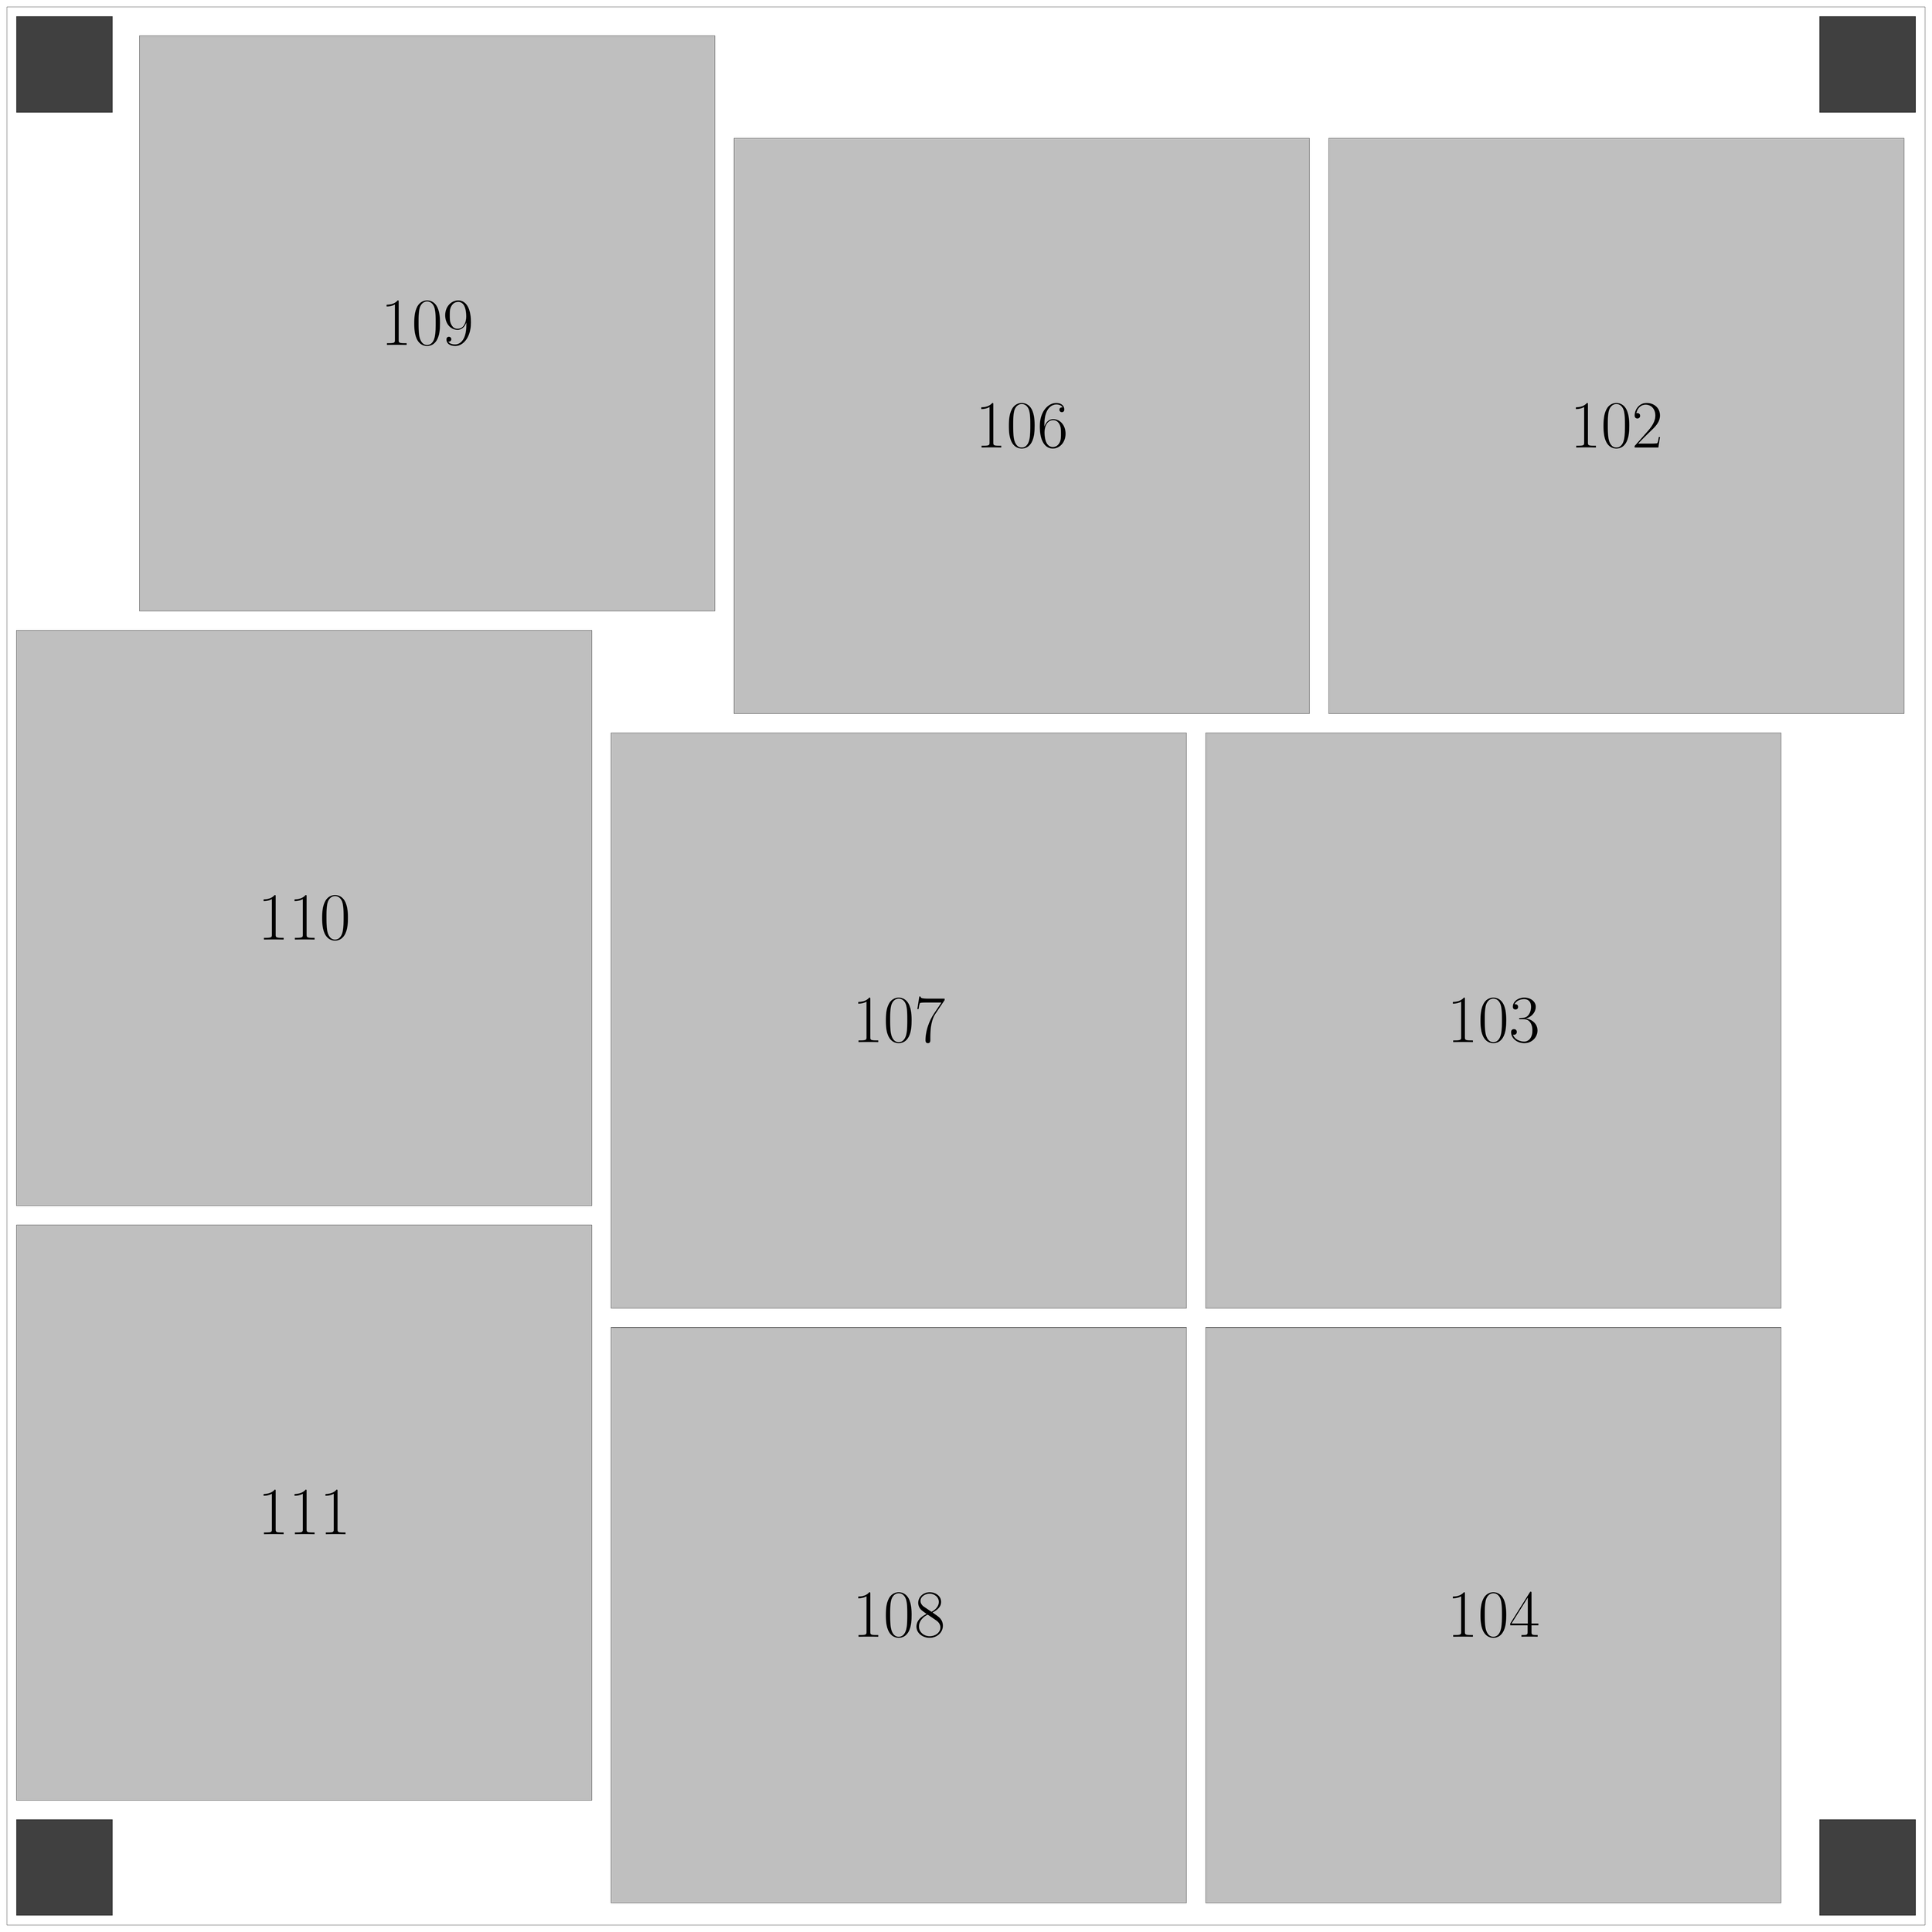
\begin{tikzpicture}\draw[black] (0,0) rectangle (100, 100);
\draw[black, fill=darkgray] (0.5,0.5) rectangle (5.5, 5.5);
\draw[black, fill=darkgray] (0.5,94.5) rectangle (5.5, 99.5);
\draw[black, fill=darkgray] (94.5,0.5) rectangle (99.5, 5.5);
\draw[black, fill=darkgray] (94.5,94.5) rectangle (99.5, 99.5);
\draw[black, fill=lightgray] (0.5,6.5) rectangle (30.5, 36.5);
\draw (15.5, 21.5) node {\fontsize{100}{120}\selectfont 111};
\draw[black, fill=lightgray] (0.5,37.5) rectangle (30.5, 67.5);
\draw (15.5, 52.5) node {\fontsize{100}{120}\selectfont 110};
\draw[black, fill=lightgray] (6.91379,68.5) rectangle (36.9138, 98.5);
\draw (21.9138, 83.5) node {\fontsize{100}{120}\selectfont 109};
\draw[black, fill=lightgray] (31.5,1.15517) rectangle (61.5, 31.1552);
\draw (46.5, 16.1552) node {\fontsize{100}{120}\selectfont 108};
\draw[black, fill=lightgray] (31.5,32.1552) rectangle (61.5, 62.1552);
\draw (46.5, 47.1552) node {\fontsize{100}{120}\selectfont 107};
\draw[black, fill=lightgray] (37.9138,63.1552) rectangle (67.9138, 93.1552);
\draw (52.9138, 78.1552) node {\fontsize{100}{120}\selectfont 106};
\draw[black, fill=lightgray] (62.5,1.15517) rectangle (92.5, 31.1552);
\draw (77.5, 16.1552) node {\fontsize{100}{120}\selectfont 104};
\draw[black, fill=lightgray] (62.5,32.1552) rectangle (92.5, 62.1552);
\draw (77.5, 47.1552) node {\fontsize{100}{120}\selectfont 103};
\draw[black, fill=lightgray] (68.9138,63.1552) rectangle (98.9138, 93.1552);
\draw (83.9138, 78.1552) node {\fontsize{100}{120}\selectfont 102};\end{tikzpicture}
}%
\newpage\clearpage
\thispagestyle{empty}
\begin{center} 
\large\textbf{3\degree Andar}\\
\vspace*{5px} 
\large
\textmd{Comprimento: 100  -  Profundidade: 100  -  Altura: 20 (cm)}\\ \end{center}
\centering
\resizebox{!}{0.9\textheight}{%
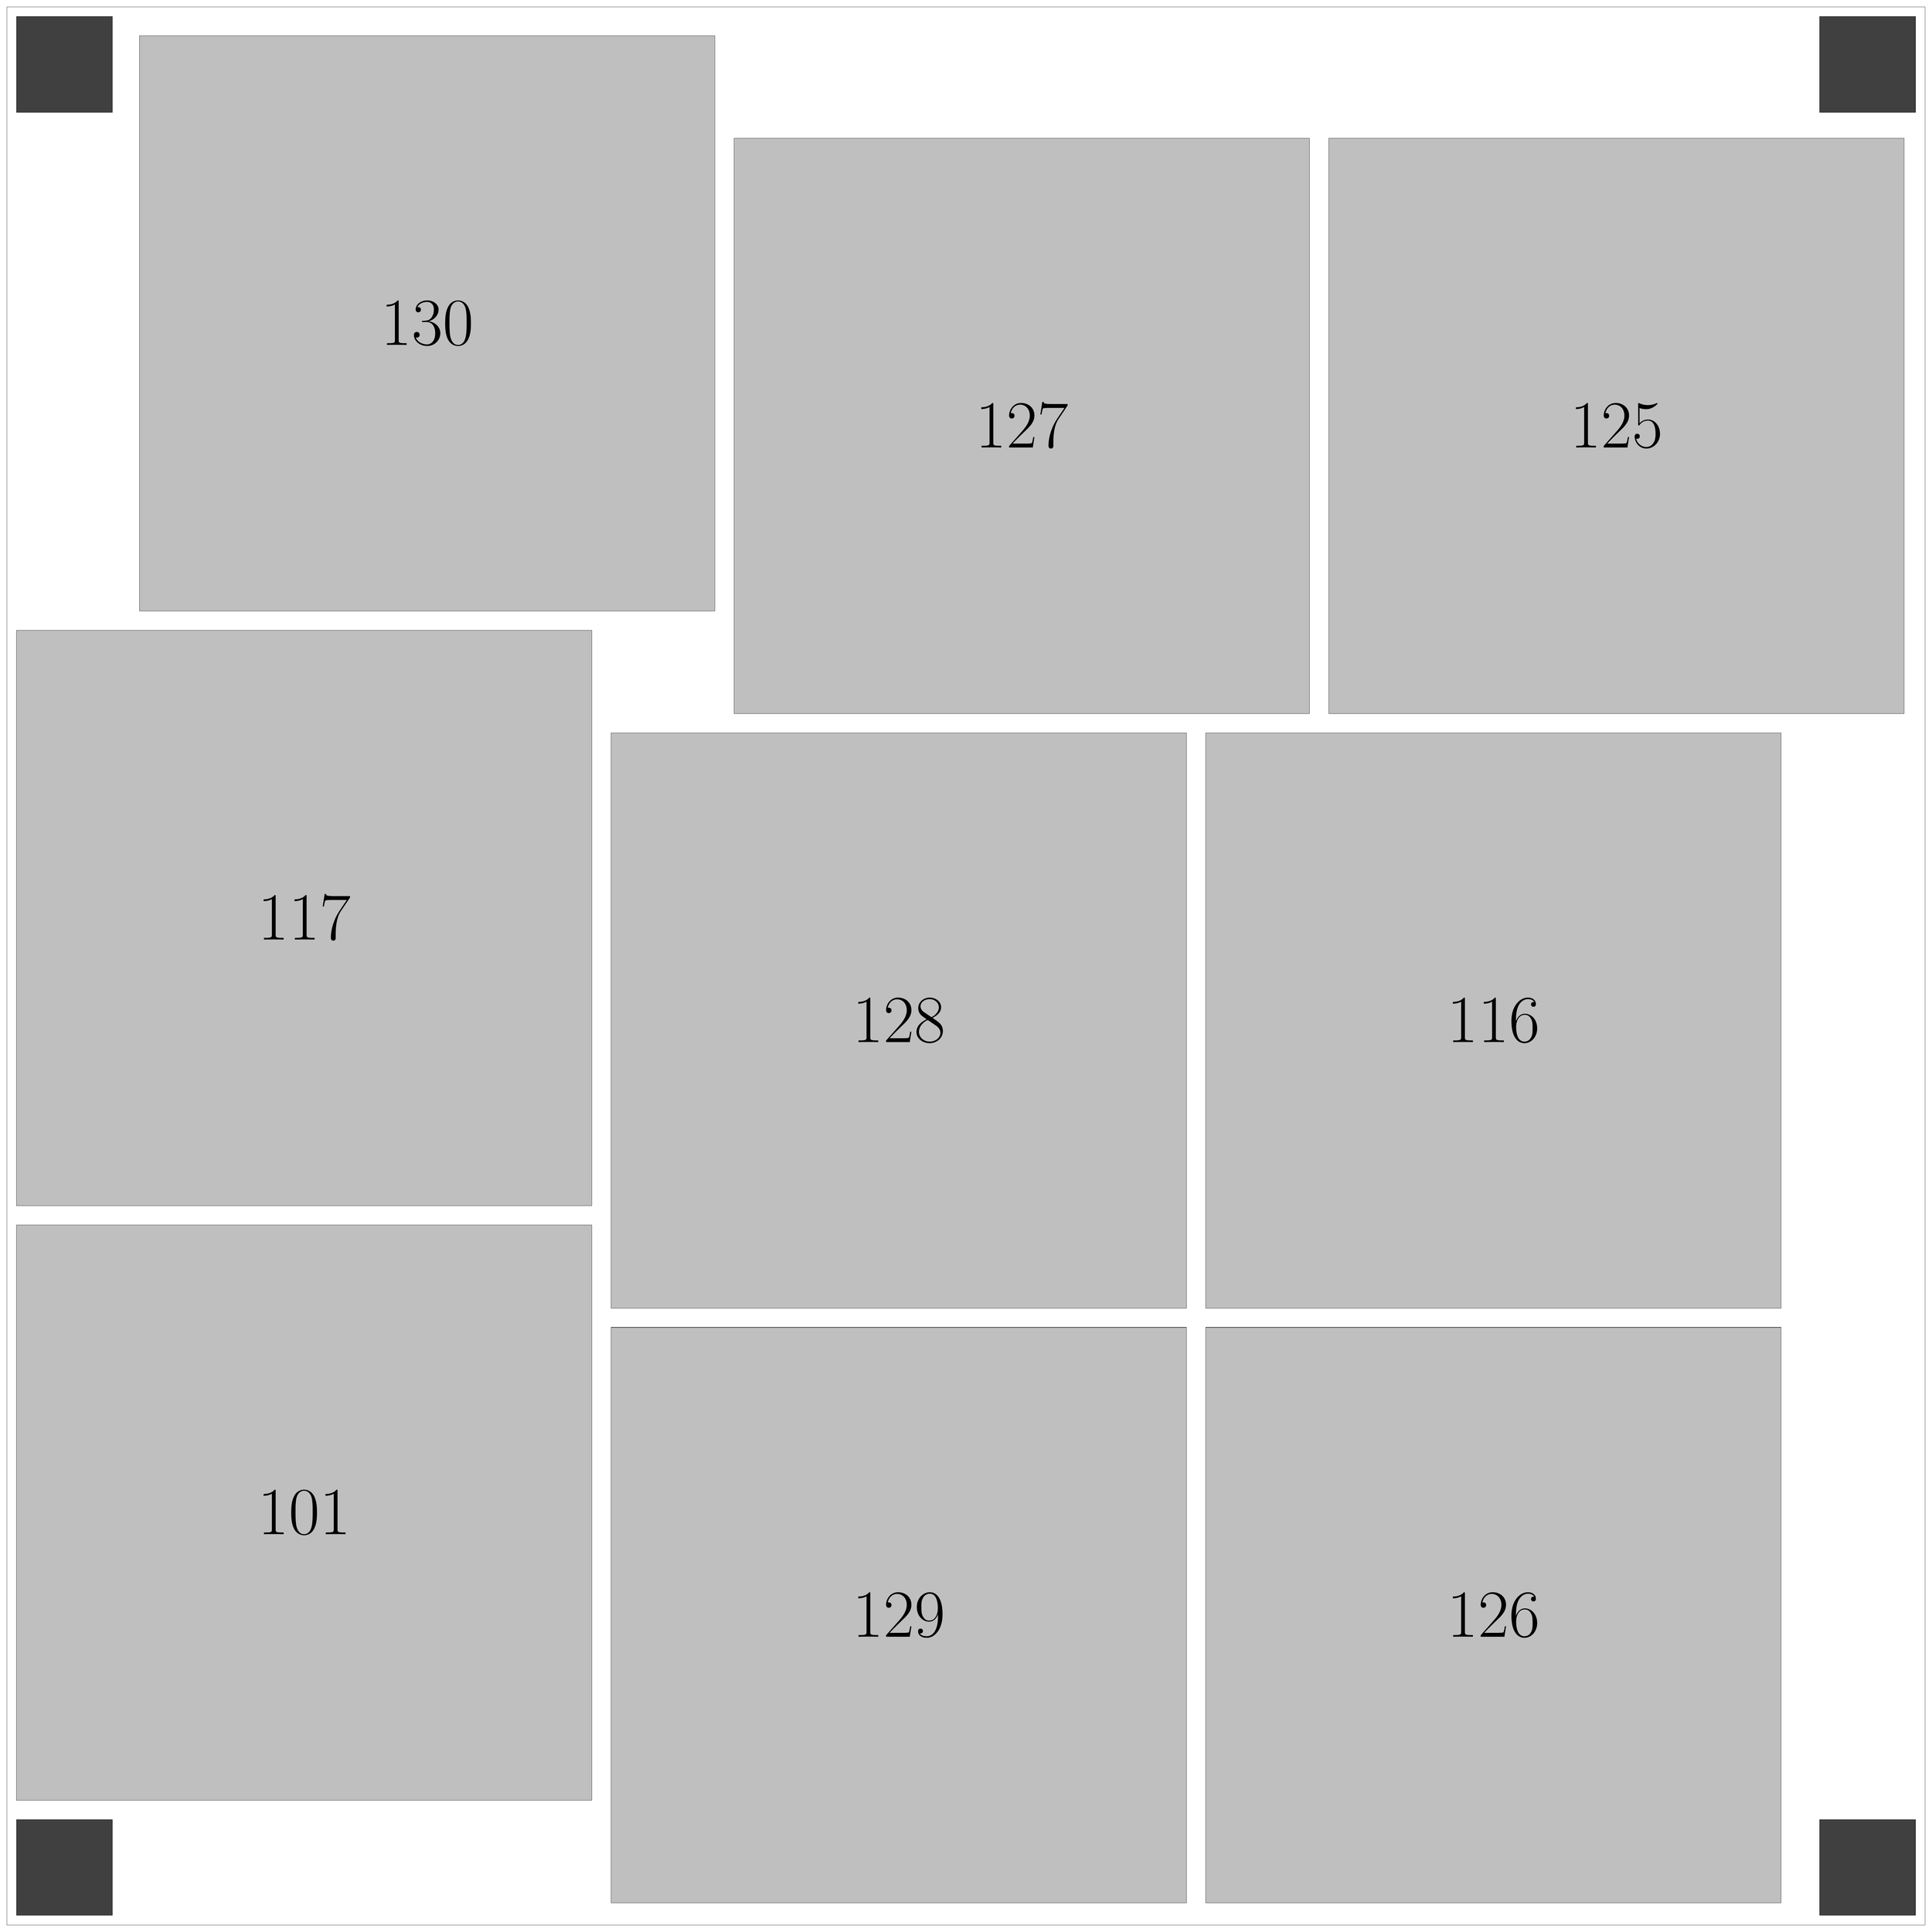
\begin{tikzpicture}\draw[black] (0,0) rectangle (100, 100);
\draw[black, fill=darkgray] (0.5,0.5) rectangle (5.5, 5.5);
\draw[black, fill=darkgray] (0.5,94.5) rectangle (5.5, 99.5);
\draw[black, fill=darkgray] (94.5,0.5) rectangle (99.5, 5.5);
\draw[black, fill=darkgray] (94.5,94.5) rectangle (99.5, 99.5);
\draw[black, fill=lightgray] (0.5,6.5) rectangle (30.5, 36.5);
\draw (15.5, 21.5) node {\fontsize{100}{120}\selectfont 101};
\draw[black, fill=lightgray] (0.5,37.5) rectangle (30.5, 67.5);
\draw (15.5, 52.5) node {\fontsize{100}{120}\selectfont 117};
\draw[black, fill=lightgray] (6.91379,68.5) rectangle (36.9138, 98.5);
\draw (21.9138, 83.5) node {\fontsize{100}{120}\selectfont 130};
\draw[black, fill=lightgray] (31.5,1.15517) rectangle (61.5, 31.1552);
\draw (46.5, 16.1552) node {\fontsize{100}{120}\selectfont 129};
\draw[black, fill=lightgray] (31.5,32.1552) rectangle (61.5, 62.1552);
\draw (46.5, 47.1552) node {\fontsize{100}{120}\selectfont 128};
\draw[black, fill=lightgray] (37.9138,63.1552) rectangle (67.9138, 93.1552);
\draw (52.9138, 78.1552) node {\fontsize{100}{120}\selectfont 127};
\draw[black, fill=lightgray] (62.5,1.15517) rectangle (92.5, 31.1552);
\draw (77.5, 16.1552) node {\fontsize{100}{120}\selectfont 126};
\draw[black, fill=lightgray] (62.5,32.1552) rectangle (92.5, 62.1552);
\draw (77.5, 47.1552) node {\fontsize{100}{120}\selectfont 116};
\draw[black, fill=lightgray] (68.9138,63.1552) rectangle (98.9138, 93.1552);
\draw (83.9138, 78.1552) node {\fontsize{100}{120}\selectfont 125};\end{tikzpicture}
}%
\newpage\clearpage
\thispagestyle{empty}
\begin{center} 
\large\textbf{4\degree Andar}\\
\vspace*{5px} 
\large
\textmd{Comprimento: 100  -  Profundidade: 100  -  Altura: 20 (cm)}\\ \end{center}
\centering
\resizebox{!}{0.9\textheight}{%
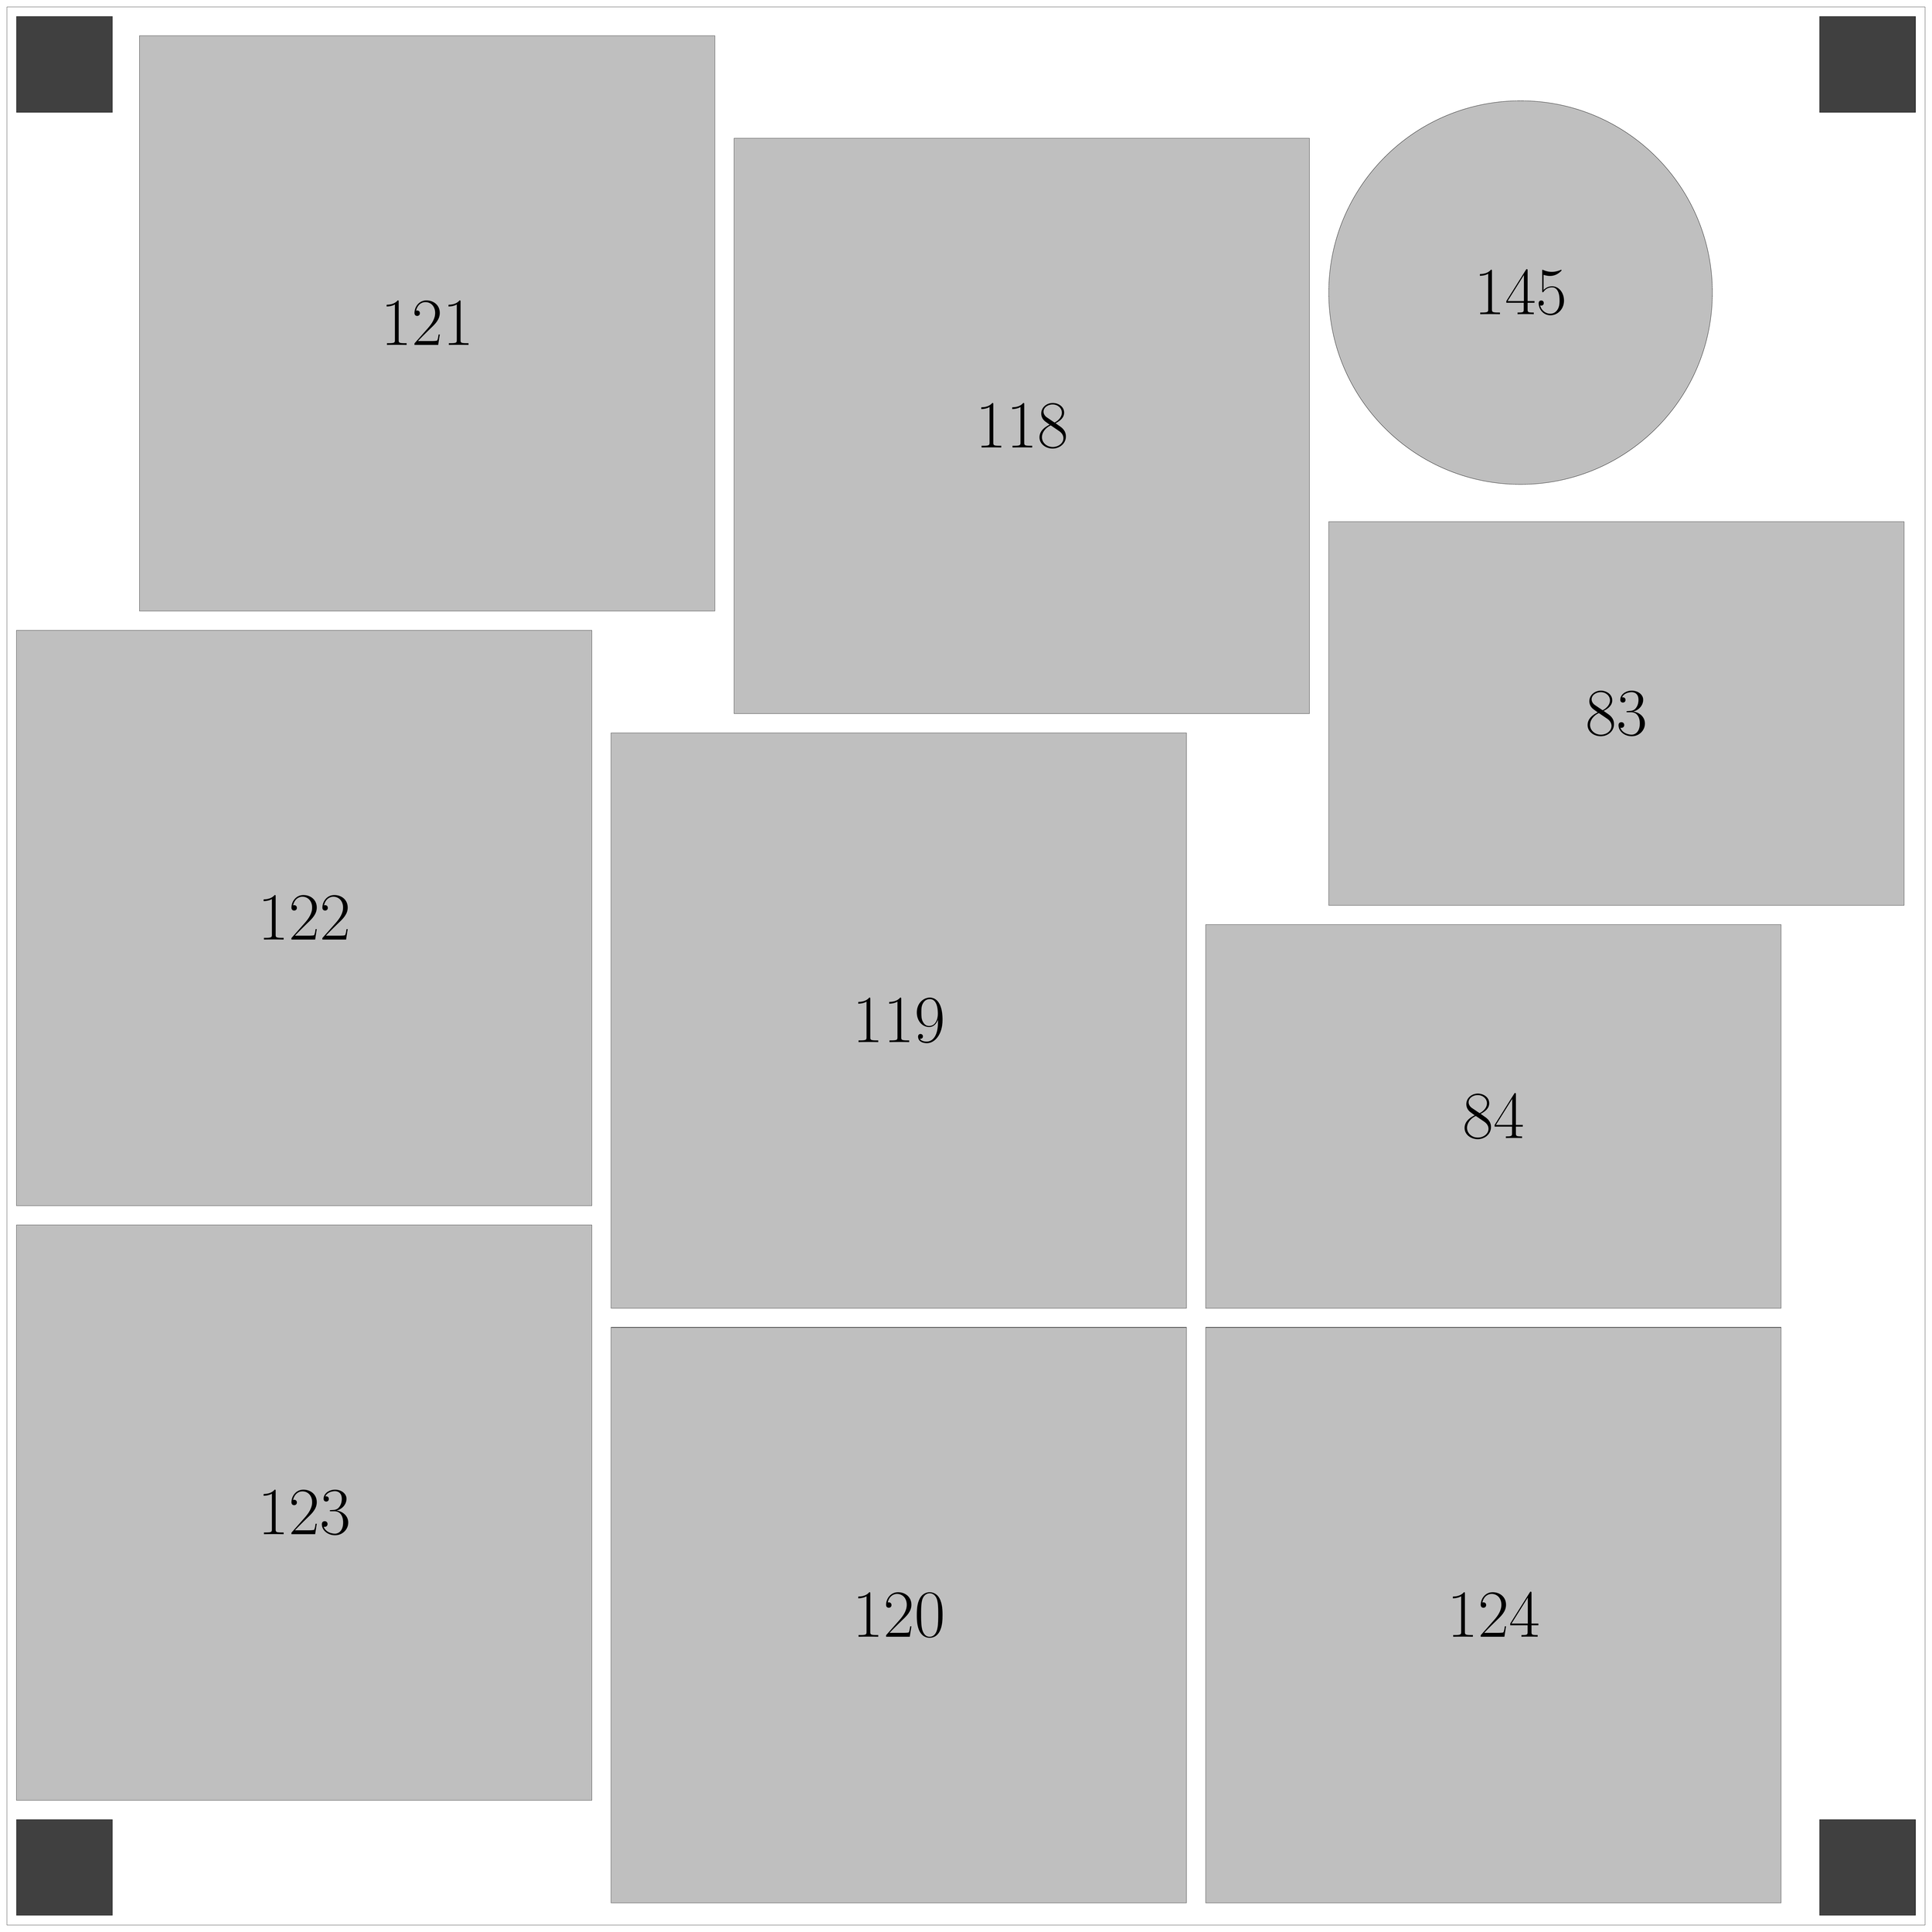
\begin{tikzpicture}\draw[black] (0,0) rectangle (100, 100);
\draw[black, fill=darkgray] (0.5,0.5) rectangle (5.5, 5.5);
\draw[black, fill=darkgray] (0.5,94.5) rectangle (5.5, 99.5);
\draw[black, fill=darkgray] (94.5,0.5) rectangle (99.5, 5.5);
\draw[black, fill=darkgray] (94.5,94.5) rectangle (99.5, 99.5);
\draw[black, fill=lightgray] (0.5,6.5) rectangle (30.5, 36.5);
\draw (15.5, 21.5) node {\fontsize{100}{120}\selectfont 123};
\draw[black, fill=lightgray] (0.5,37.5) rectangle (30.5, 67.5);
\draw (15.5, 52.5) node {\fontsize{100}{120}\selectfont 122};
\draw[black, fill=lightgray] (6.91379,68.5) rectangle (36.9138, 98.5);
\draw (21.9138, 83.5) node {\fontsize{100}{120}\selectfont 121};
\draw[black, fill=lightgray] (31.5,1.15517) rectangle (61.5, 31.1552);
\draw (46.5, 16.1552) node {\fontsize{100}{120}\selectfont 120};
\draw[black, fill=lightgray] (31.5,32.1552) rectangle (61.5, 62.1552);
\draw (46.5, 47.1552) node {\fontsize{100}{120}\selectfont 119};
\draw[black, fill=lightgray] (37.9138,63.1552) rectangle (67.9138, 93.1552);
\draw (52.9138, 78.1552) node {\fontsize{100}{120}\selectfont 118};
\draw[black, fill=lightgray] (62.5,1.15517) rectangle (92.5, 31.1552);
\draw (77.5, 16.1552) node {\fontsize{100}{120}\selectfont 124};
\draw[black, fill=lightgray] (62.5,32.1552) rectangle (92.5, 52.1552);
\draw (77.5, 42.1552) node {\fontsize{100}{120}\selectfont 84};
\draw[black, fill=lightgray] (68.9138,53.1552) rectangle (98.9138, 73.1552);
\draw (83.9138, 63.1552) node {\fontsize{100}{120}\selectfont 83};
\draw[black, fill=lightgray] (78.9138,85.1034) circle (10);
\draw (78.9138, 85.1034) node {\fontsize{100}{120}\selectfont 145};\end{tikzpicture}
}%
\newpage\clearpage
\thispagestyle{empty}
\begin{center} 
\large\textbf{5\degree Andar}\\
\vspace*{5px} 
\large
\textmd{Comprimento: 100  -  Profundidade: 100  -  Altura: 20 (cm)}\\ \end{center}
\centering
\resizebox{!}{0.9\textheight}{%
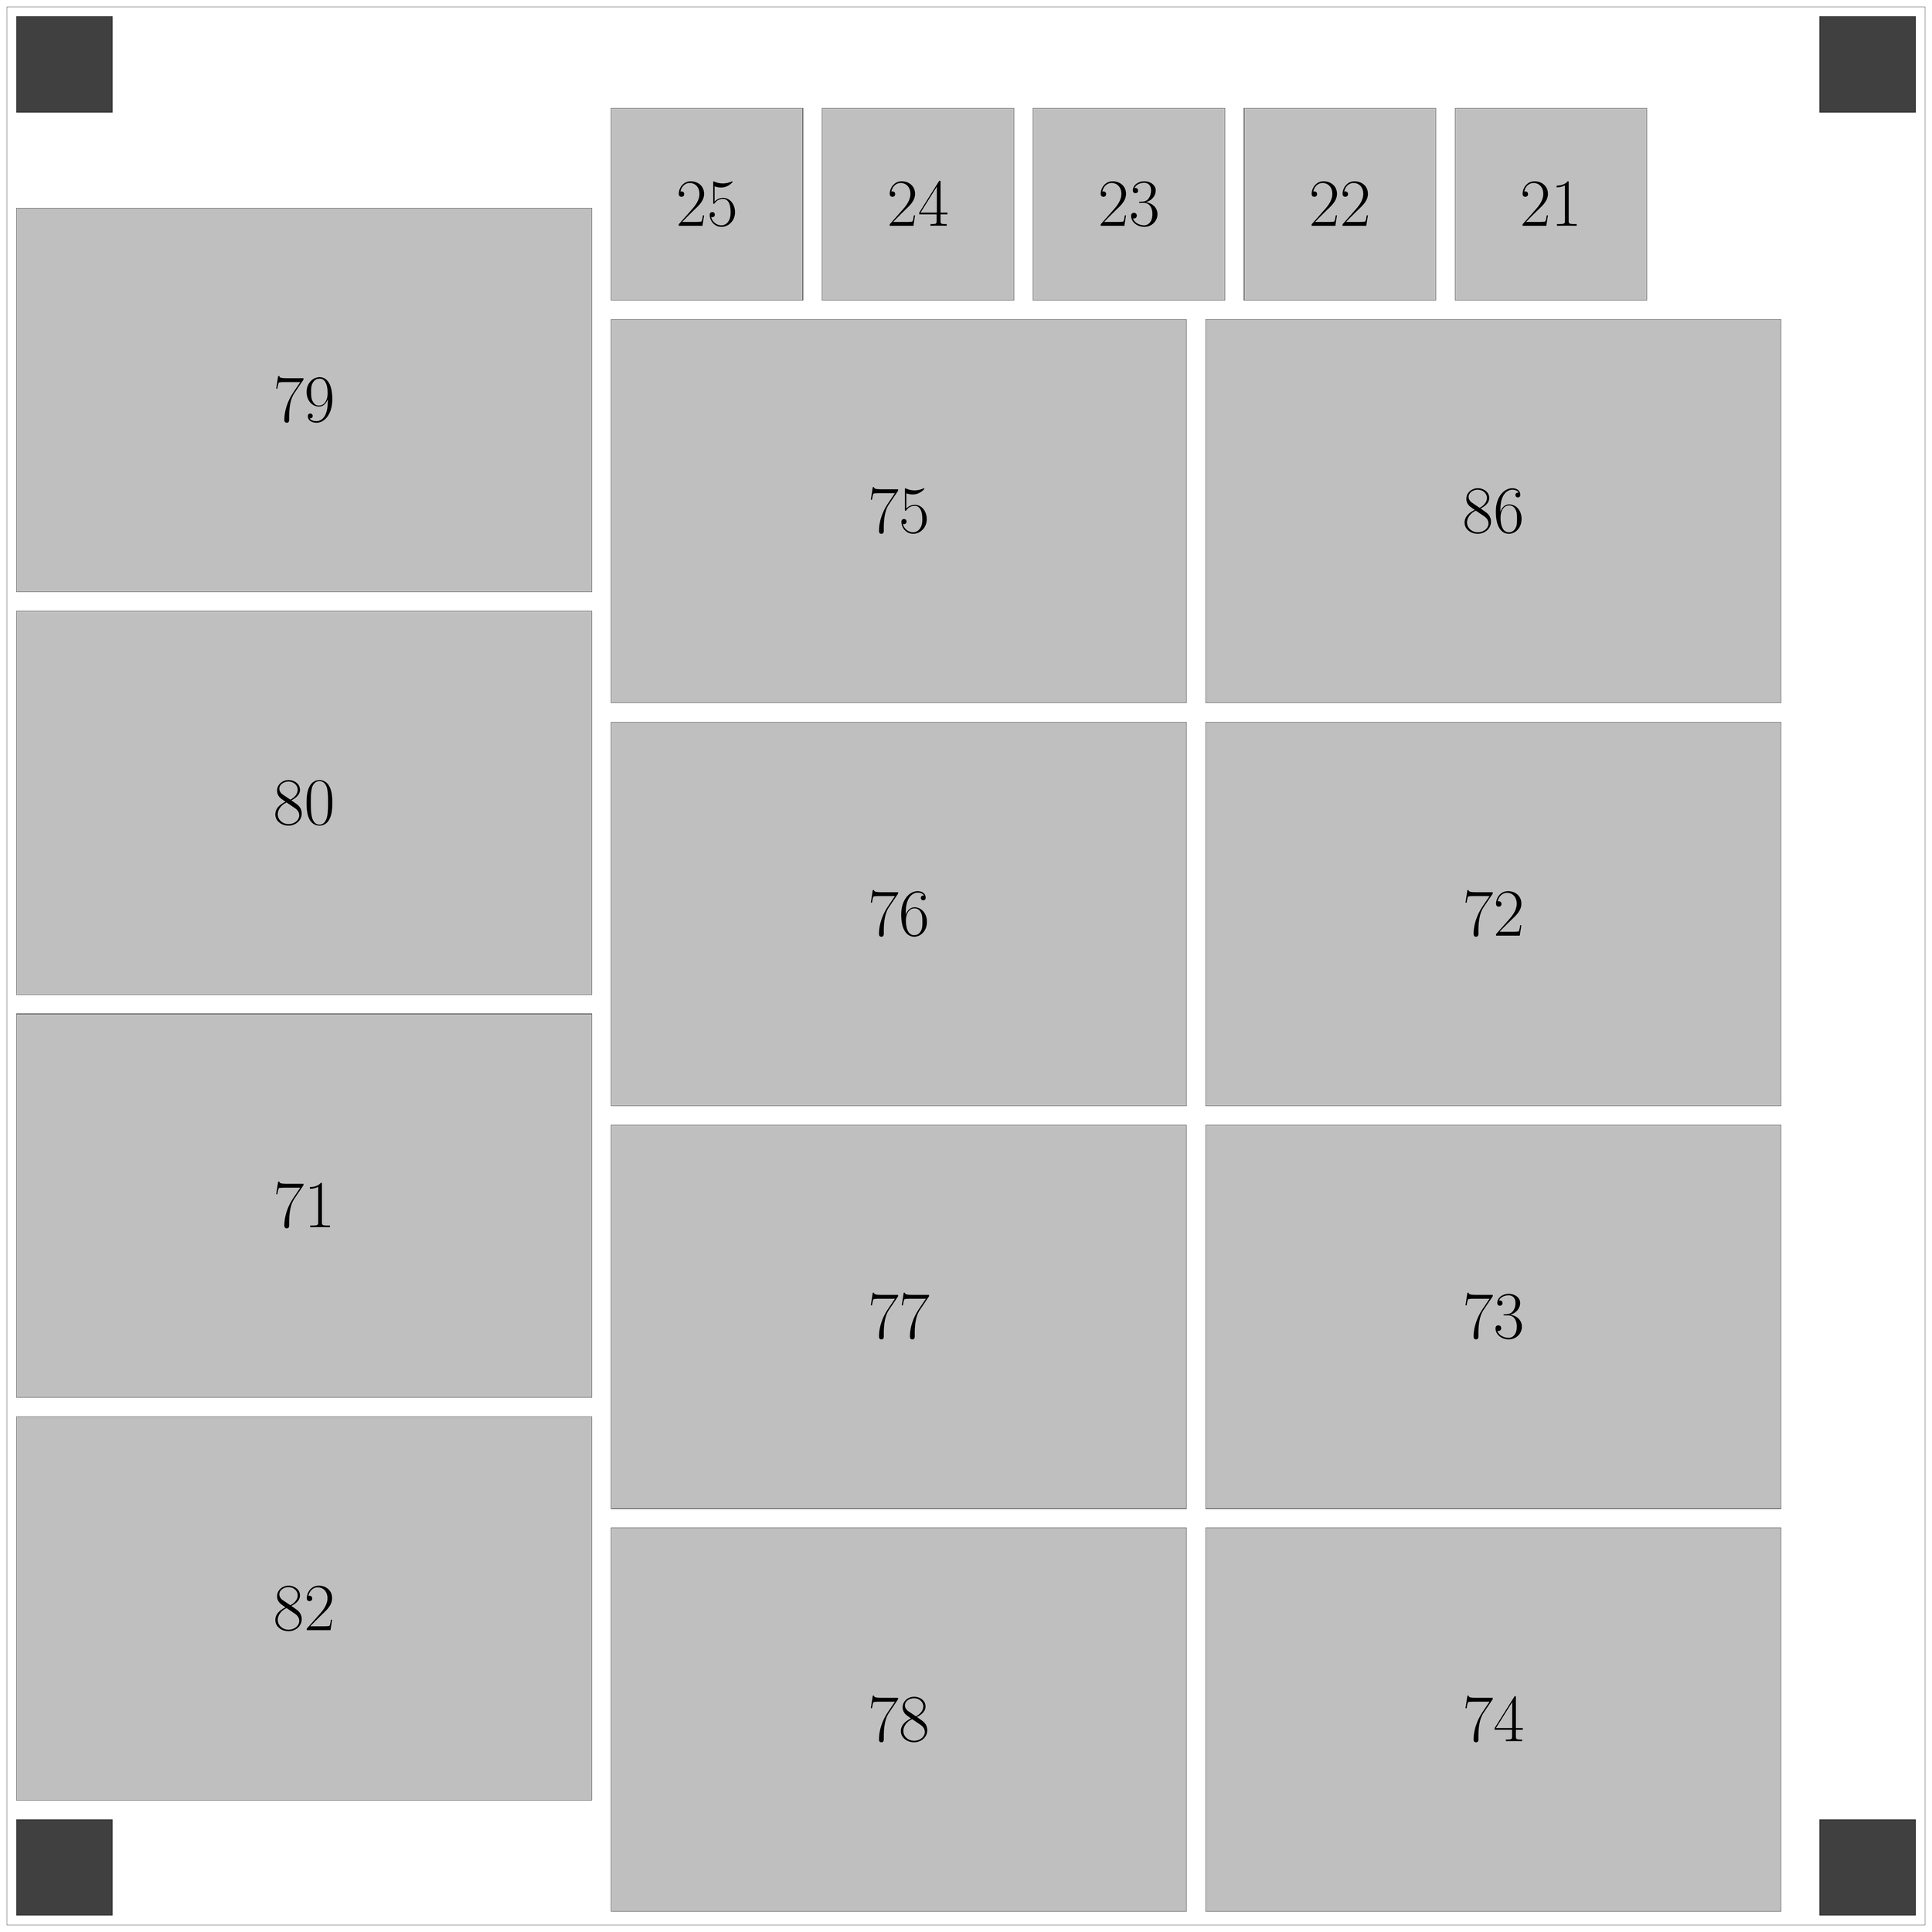
\begin{tikzpicture}\draw[black] (0,0) rectangle (100, 100);
\draw[black, fill=darkgray] (0.5,0.5) rectangle (5.5, 5.5);
\draw[black, fill=darkgray] (0.5,94.5) rectangle (5.5, 99.5);
\draw[black, fill=darkgray] (94.5,0.5) rectangle (99.5, 5.5);
\draw[black, fill=darkgray] (94.5,94.5) rectangle (99.5, 99.5);
\draw[black, fill=lightgray] (0.5,6.5) rectangle (30.5, 26.5);
\draw (15.5, 16.5) node {\fontsize{100}{120}\selectfont 82};
\draw[black, fill=lightgray] (0.5,27.5) rectangle (30.5, 47.5);
\draw (15.5, 37.5) node {\fontsize{100}{120}\selectfont 71};
\draw[black, fill=lightgray] (0.5,48.5) rectangle (30.5, 68.5);
\draw (15.5, 58.5) node {\fontsize{100}{120}\selectfont 80};
\draw[black, fill=lightgray] (0.5,69.5) rectangle (30.5, 89.5);
\draw (15.5, 79.5) node {\fontsize{100}{120}\selectfont 79};
\draw[black, fill=lightgray] (31.5,0.706897) rectangle (61.5, 20.7069);
\draw (46.5, 10.7069) node {\fontsize{100}{120}\selectfont 78};
\draw[black, fill=lightgray] (31.5,21.7069) rectangle (61.5, 41.7069);
\draw (46.5, 31.7069) node {\fontsize{100}{120}\selectfont 77};
\draw[black, fill=lightgray] (31.5,42.7069) rectangle (61.5, 62.7069);
\draw (46.5, 52.7069) node {\fontsize{100}{120}\selectfont 76};
\draw[black, fill=lightgray] (31.5,63.7069) rectangle (61.5, 83.7069);
\draw (46.5, 73.7069) node {\fontsize{100}{120}\selectfont 75};
\draw[black, fill=lightgray] (62.5,0.706897) rectangle (92.5, 20.7069);
\draw (77.5, 10.7069) node {\fontsize{100}{120}\selectfont 74};
\draw[black, fill=lightgray] (62.5,21.7069) rectangle (92.5, 41.7069);
\draw (77.5, 31.7069) node {\fontsize{100}{120}\selectfont 73};
\draw[black, fill=lightgray] (62.5,42.7069) rectangle (92.5, 62.7069);
\draw (77.5, 52.7069) node {\fontsize{100}{120}\selectfont 72};
\draw[black, fill=lightgray] (62.5,63.7069) rectangle (92.5, 83.7069);
\draw (77.5, 73.7069) node {\fontsize{100}{120}\selectfont 86};
\draw[black, fill=lightgray] (31.5,84.7069) rectangle (41.5, 94.7069);
\draw (36.5, 89.7069) node {\fontsize{100}{120}\selectfont 25};
\draw[black, fill=lightgray] (42.5,84.7069) rectangle (52.5, 94.7069);
\draw (47.5, 89.7069) node {\fontsize{100}{120}\selectfont 24};
\draw[black, fill=lightgray] (53.5,84.7069) rectangle (63.5, 94.7069);
\draw (58.5, 89.7069) node {\fontsize{100}{120}\selectfont 23};
\draw[black, fill=lightgray] (64.5,84.7069) rectangle (74.5, 94.7069);
\draw (69.5, 89.7069) node {\fontsize{100}{120}\selectfont 22};
\draw[black, fill=lightgray] (75.5,84.7069) rectangle (85.5, 94.7069);
\draw (80.5, 89.7069) node {\fontsize{100}{120}\selectfont 21};\end{tikzpicture}
}%
\newpage\clearpage
\thispagestyle{empty}
\begin{center} 
\large\textbf{6\degree Andar}\\
\vspace*{5px} 
\large
\textmd{Comprimento: 100  -  Profundidade: 100  -  Altura: 20 (cm)}\\ \end{center}
\centering
\resizebox{!}{0.9\textheight}{%
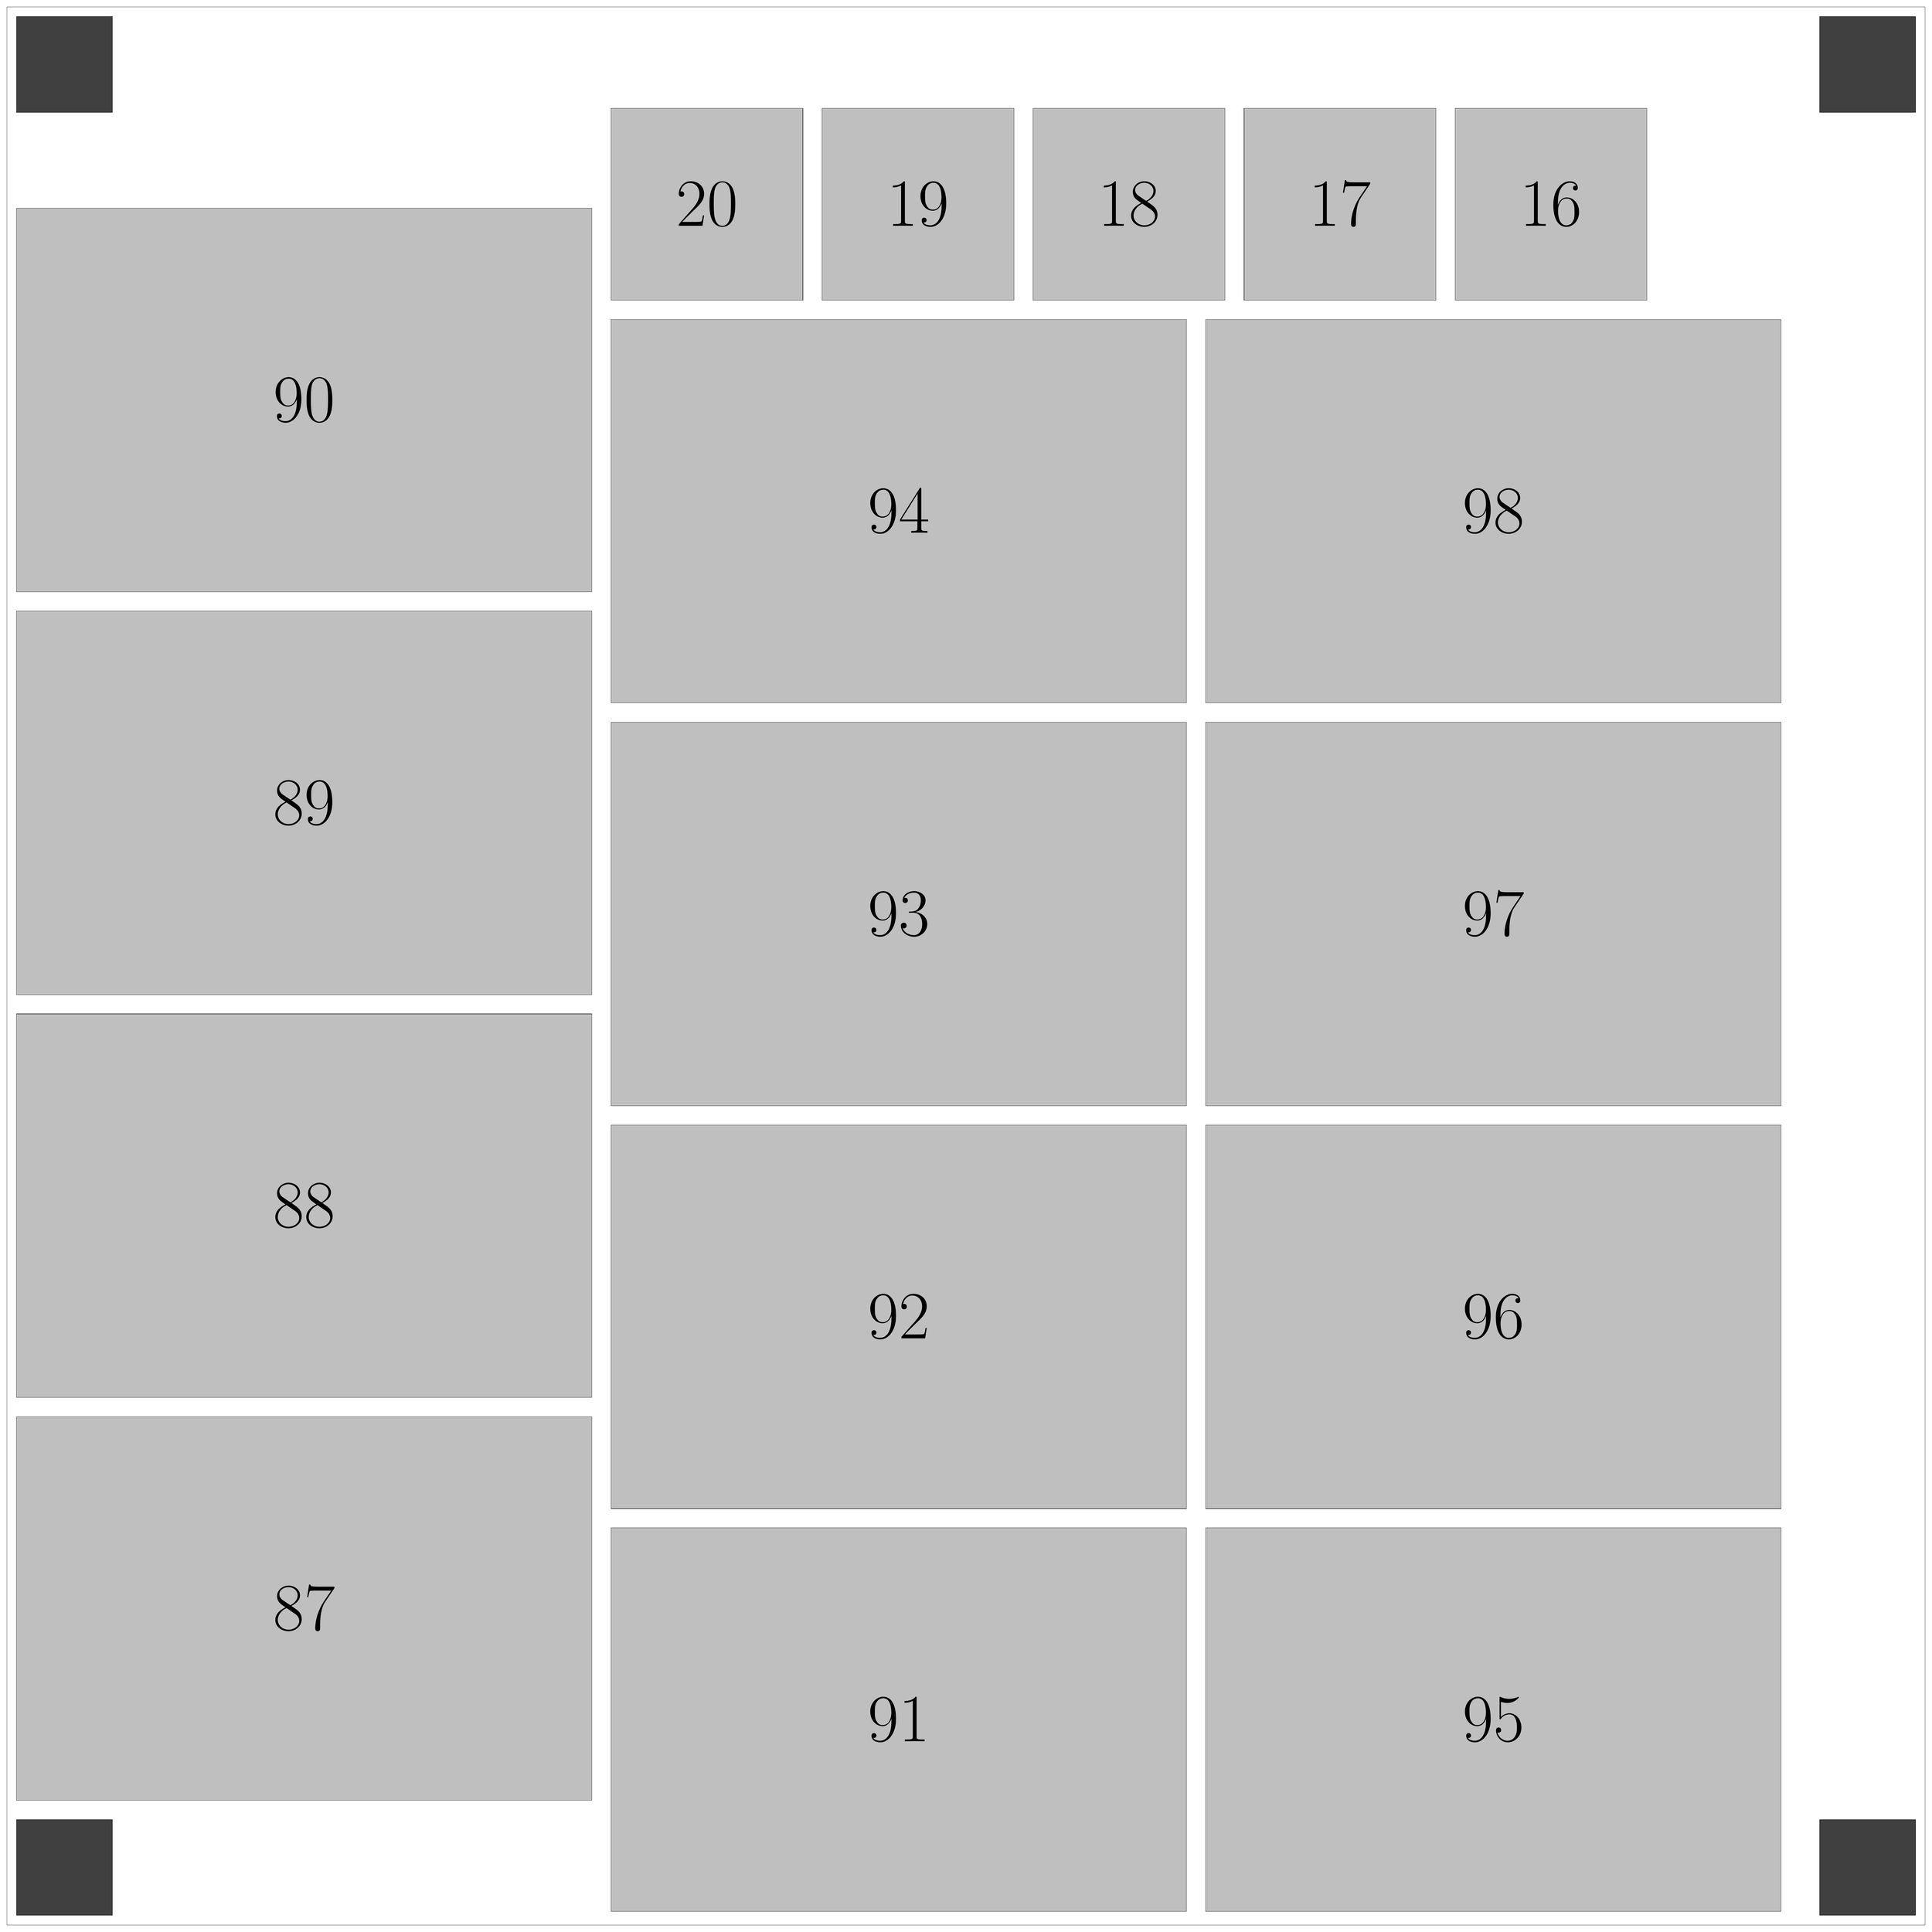
\begin{tikzpicture}\draw[black] (0,0) rectangle (100, 100);
\draw[black, fill=darkgray] (0.5,0.5) rectangle (5.5, 5.5);
\draw[black, fill=darkgray] (0.5,94.5) rectangle (5.5, 99.5);
\draw[black, fill=darkgray] (94.5,0.5) rectangle (99.5, 5.5);
\draw[black, fill=darkgray] (94.5,94.5) rectangle (99.5, 99.5);
\draw[black, fill=lightgray] (0.5,6.5) rectangle (30.5, 26.5);
\draw (15.5, 16.5) node {\fontsize{100}{120}\selectfont 87};
\draw[black, fill=lightgray] (0.5,27.5) rectangle (30.5, 47.5);
\draw (15.5, 37.5) node {\fontsize{100}{120}\selectfont 88};
\draw[black, fill=lightgray] (0.5,48.5) rectangle (30.5, 68.5);
\draw (15.5, 58.5) node {\fontsize{100}{120}\selectfont 89};
\draw[black, fill=lightgray] (0.5,69.5) rectangle (30.5, 89.5);
\draw (15.5, 79.5) node {\fontsize{100}{120}\selectfont 90};
\draw[black, fill=lightgray] (31.5,0.706897) rectangle (61.5, 20.7069);
\draw (46.5, 10.7069) node {\fontsize{100}{120}\selectfont 91};
\draw[black, fill=lightgray] (31.5,21.7069) rectangle (61.5, 41.7069);
\draw (46.5, 31.7069) node {\fontsize{100}{120}\selectfont 92};
\draw[black, fill=lightgray] (31.5,42.7069) rectangle (61.5, 62.7069);
\draw (46.5, 52.7069) node {\fontsize{100}{120}\selectfont 93};
\draw[black, fill=lightgray] (31.5,63.7069) rectangle (61.5, 83.7069);
\draw (46.5, 73.7069) node {\fontsize{100}{120}\selectfont 94};
\draw[black, fill=lightgray] (62.5,0.706897) rectangle (92.5, 20.7069);
\draw (77.5, 10.7069) node {\fontsize{100}{120}\selectfont 95};
\draw[black, fill=lightgray] (62.5,21.7069) rectangle (92.5, 41.7069);
\draw (77.5, 31.7069) node {\fontsize{100}{120}\selectfont 96};
\draw[black, fill=lightgray] (62.5,42.7069) rectangle (92.5, 62.7069);
\draw (77.5, 52.7069) node {\fontsize{100}{120}\selectfont 97};
\draw[black, fill=lightgray] (62.5,63.7069) rectangle (92.5, 83.7069);
\draw (77.5, 73.7069) node {\fontsize{100}{120}\selectfont 98};
\draw[black, fill=lightgray] (31.5,84.7069) rectangle (41.5, 94.7069);
\draw (36.5, 89.7069) node {\fontsize{100}{120}\selectfont 20};
\draw[black, fill=lightgray] (42.5,84.7069) rectangle (52.5, 94.7069);
\draw (47.5, 89.7069) node {\fontsize{100}{120}\selectfont 19};
\draw[black, fill=lightgray] (53.5,84.7069) rectangle (63.5, 94.7069);
\draw (58.5, 89.7069) node {\fontsize{100}{120}\selectfont 18};
\draw[black, fill=lightgray] (64.5,84.7069) rectangle (74.5, 94.7069);
\draw (69.5, 89.7069) node {\fontsize{100}{120}\selectfont 17};
\draw[black, fill=lightgray] (75.5,84.7069) rectangle (85.5, 94.7069);
\draw (80.5, 89.7069) node {\fontsize{100}{120}\selectfont 16};\end{tikzpicture}
}%
\newpage\clearpage
\thispagestyle{empty}
\begin{center} 
\large\textbf{7\degree Andar}\\
\vspace*{5px} 
\large
\textmd{Comprimento: 100  -  Profundidade: 100  -  Altura: 20 (cm)}\\ \end{center}
\centering
\resizebox{!}{0.9\textheight}{%
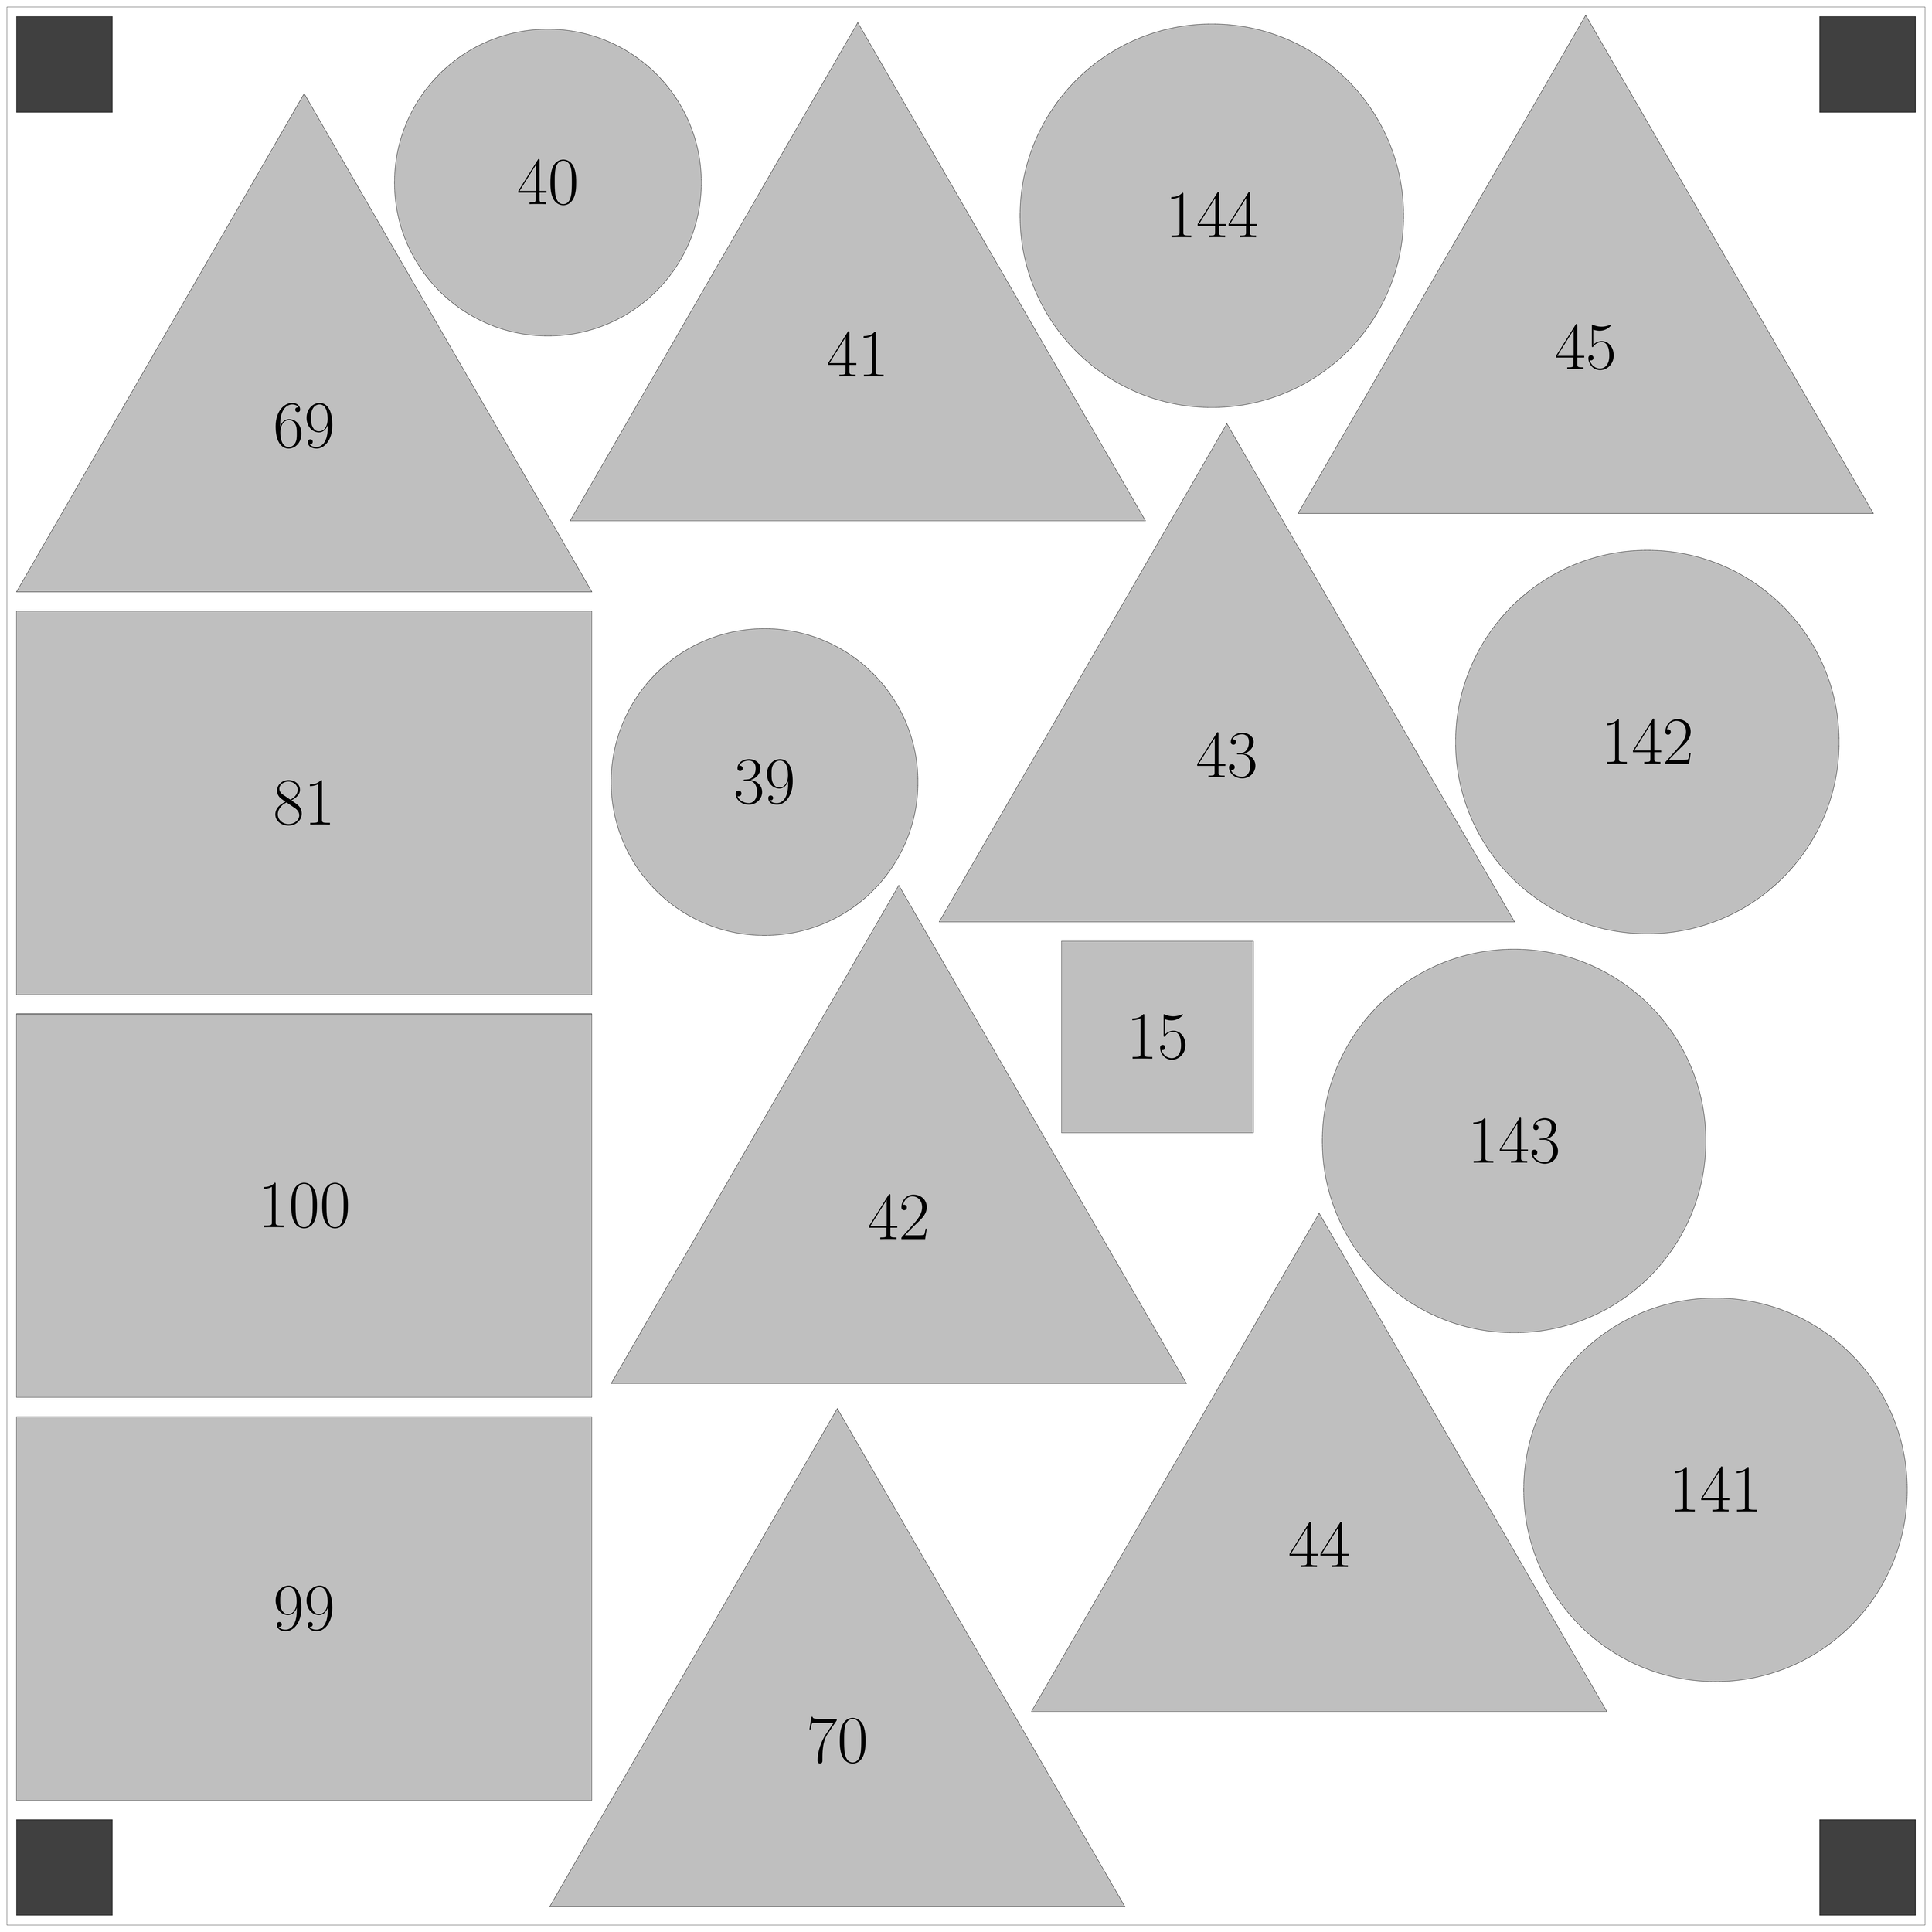
\begin{tikzpicture}\draw[black] (0,0) rectangle (100, 100);
\draw[black, fill=darkgray] (0.5,0.5) rectangle (5.5, 5.5);
\draw[black, fill=darkgray] (0.5,94.5) rectangle (5.5, 99.5);
\draw[black, fill=darkgray] (94.5,0.5) rectangle (99.5, 5.5);
\draw[black, fill=darkgray] (94.5,94.5) rectangle (99.5, 99.5);
\draw[black, fill=lightgray] (0.5,6.5) rectangle (30.5, 26.5);
\draw (15.5, 16.5) node {\fontsize{100}{120}\selectfont 99};
\draw[black, fill=lightgray] (0.5,27.5) rectangle (30.5, 47.5);
\draw (15.5, 37.5) node {\fontsize{100}{120}\selectfont 100};
\draw[black, fill=lightgray] (0.5,48.5) rectangle (30.5, 68.5);
\draw (15.5, 58.5) node {\fontsize{100}{120}\selectfont 81};
\draw[black, fill=lightgray] (0.5,69.5) -- (30.5, 69.5) -- (15.5, 95.4808) -- cycle;
\draw (15.5, 78.1603) node {\fontsize{100}{120}\selectfont 69};
\draw[black, fill=lightgray] (28.2931,0.945492) -- (58.2931, 0.945492) -- (43.2931, 26.9263) -- cycle;
\draw (43.2931, 9.60575) node {\fontsize{100}{120}\selectfont 70};
\draw[black, fill=lightgray] (29.3621,73.203) -- (59.3621, 73.203) -- (44.3621, 99.1838) -- cycle;
\draw (44.3621, 81.8633) node {\fontsize{100}{120}\selectfont 41};
\draw[black, fill=lightgray] (31.5,28.2241) -- (61.5, 28.2241) -- (46.5, 54.2049) -- cycle;
\draw (46.5, 36.8844) node {\fontsize{100}{120}\selectfont 42};
\draw[black, fill=lightgray] (48.6034,52.2937) -- (78.6034, 52.2937) -- (63.6034, 78.2744) -- cycle;
\draw (63.6034, 60.9539) node {\fontsize{100}{120}\selectfont 43};
\draw[black, fill=lightgray] (53.4138,11.1288) -- (83.4138, 11.1288) -- (68.4138, 37.1095) -- cycle;
\draw (68.4138, 19.789) node {\fontsize{100}{120}\selectfont 44};
\draw[black, fill=lightgray] (67.3103,73.586) -- (97.3103, 73.586) -- (82.3103, 99.5667) -- cycle;
\draw (82.3103, 82.2462) node {\fontsize{100}{120}\selectfont 45};
\draw[black, fill=lightgray] (62.8188,89.1111) circle (10);
\draw (62.8188, 89.1111) node {\fontsize{100}{120}\selectfont 144};
\draw[black, fill=lightgray] (78.576,40.874) circle (10);
\draw (78.576, 40.874) node {\fontsize{100}{120}\selectfont 143};
\draw[black, fill=lightgray] (85.5243,61.6724) circle (10);
\draw (85.5243, 61.6724) node {\fontsize{100}{120}\selectfont 142};
\draw[black, fill=lightgray] (89.076,22.6875) circle (10);
\draw (89.076, 22.6875) node {\fontsize{100}{120}\selectfont 141};
\draw[black, fill=lightgray] (28.206,90.8393) circle (8);
\draw (28.206, 90.8393) node {\fontsize{100}{120}\selectfont 40};
\draw[black, fill=lightgray] (39.5,59.5862) circle (8);
\draw (39.5, 59.5862) node {\fontsize{100}{120}\selectfont 39};
\draw[black, fill=lightgray] (54.9828,41.2937) rectangle (64.9828, 51.2937);
\draw (59.9828, 46.2937) node {\fontsize{100}{120}\selectfont 15};\end{tikzpicture}
}%
\newpage\clearpage
\thispagestyle{empty}
\begin{center} 
\large\textbf{8\degree Andar}\\
\vspace*{5px} 
\large
\textmd{Comprimento: 100  -  Profundidade: 100  -  Altura: 20 (cm)}\\ \end{center}
\centering
\resizebox{!}{0.9\textheight}{%
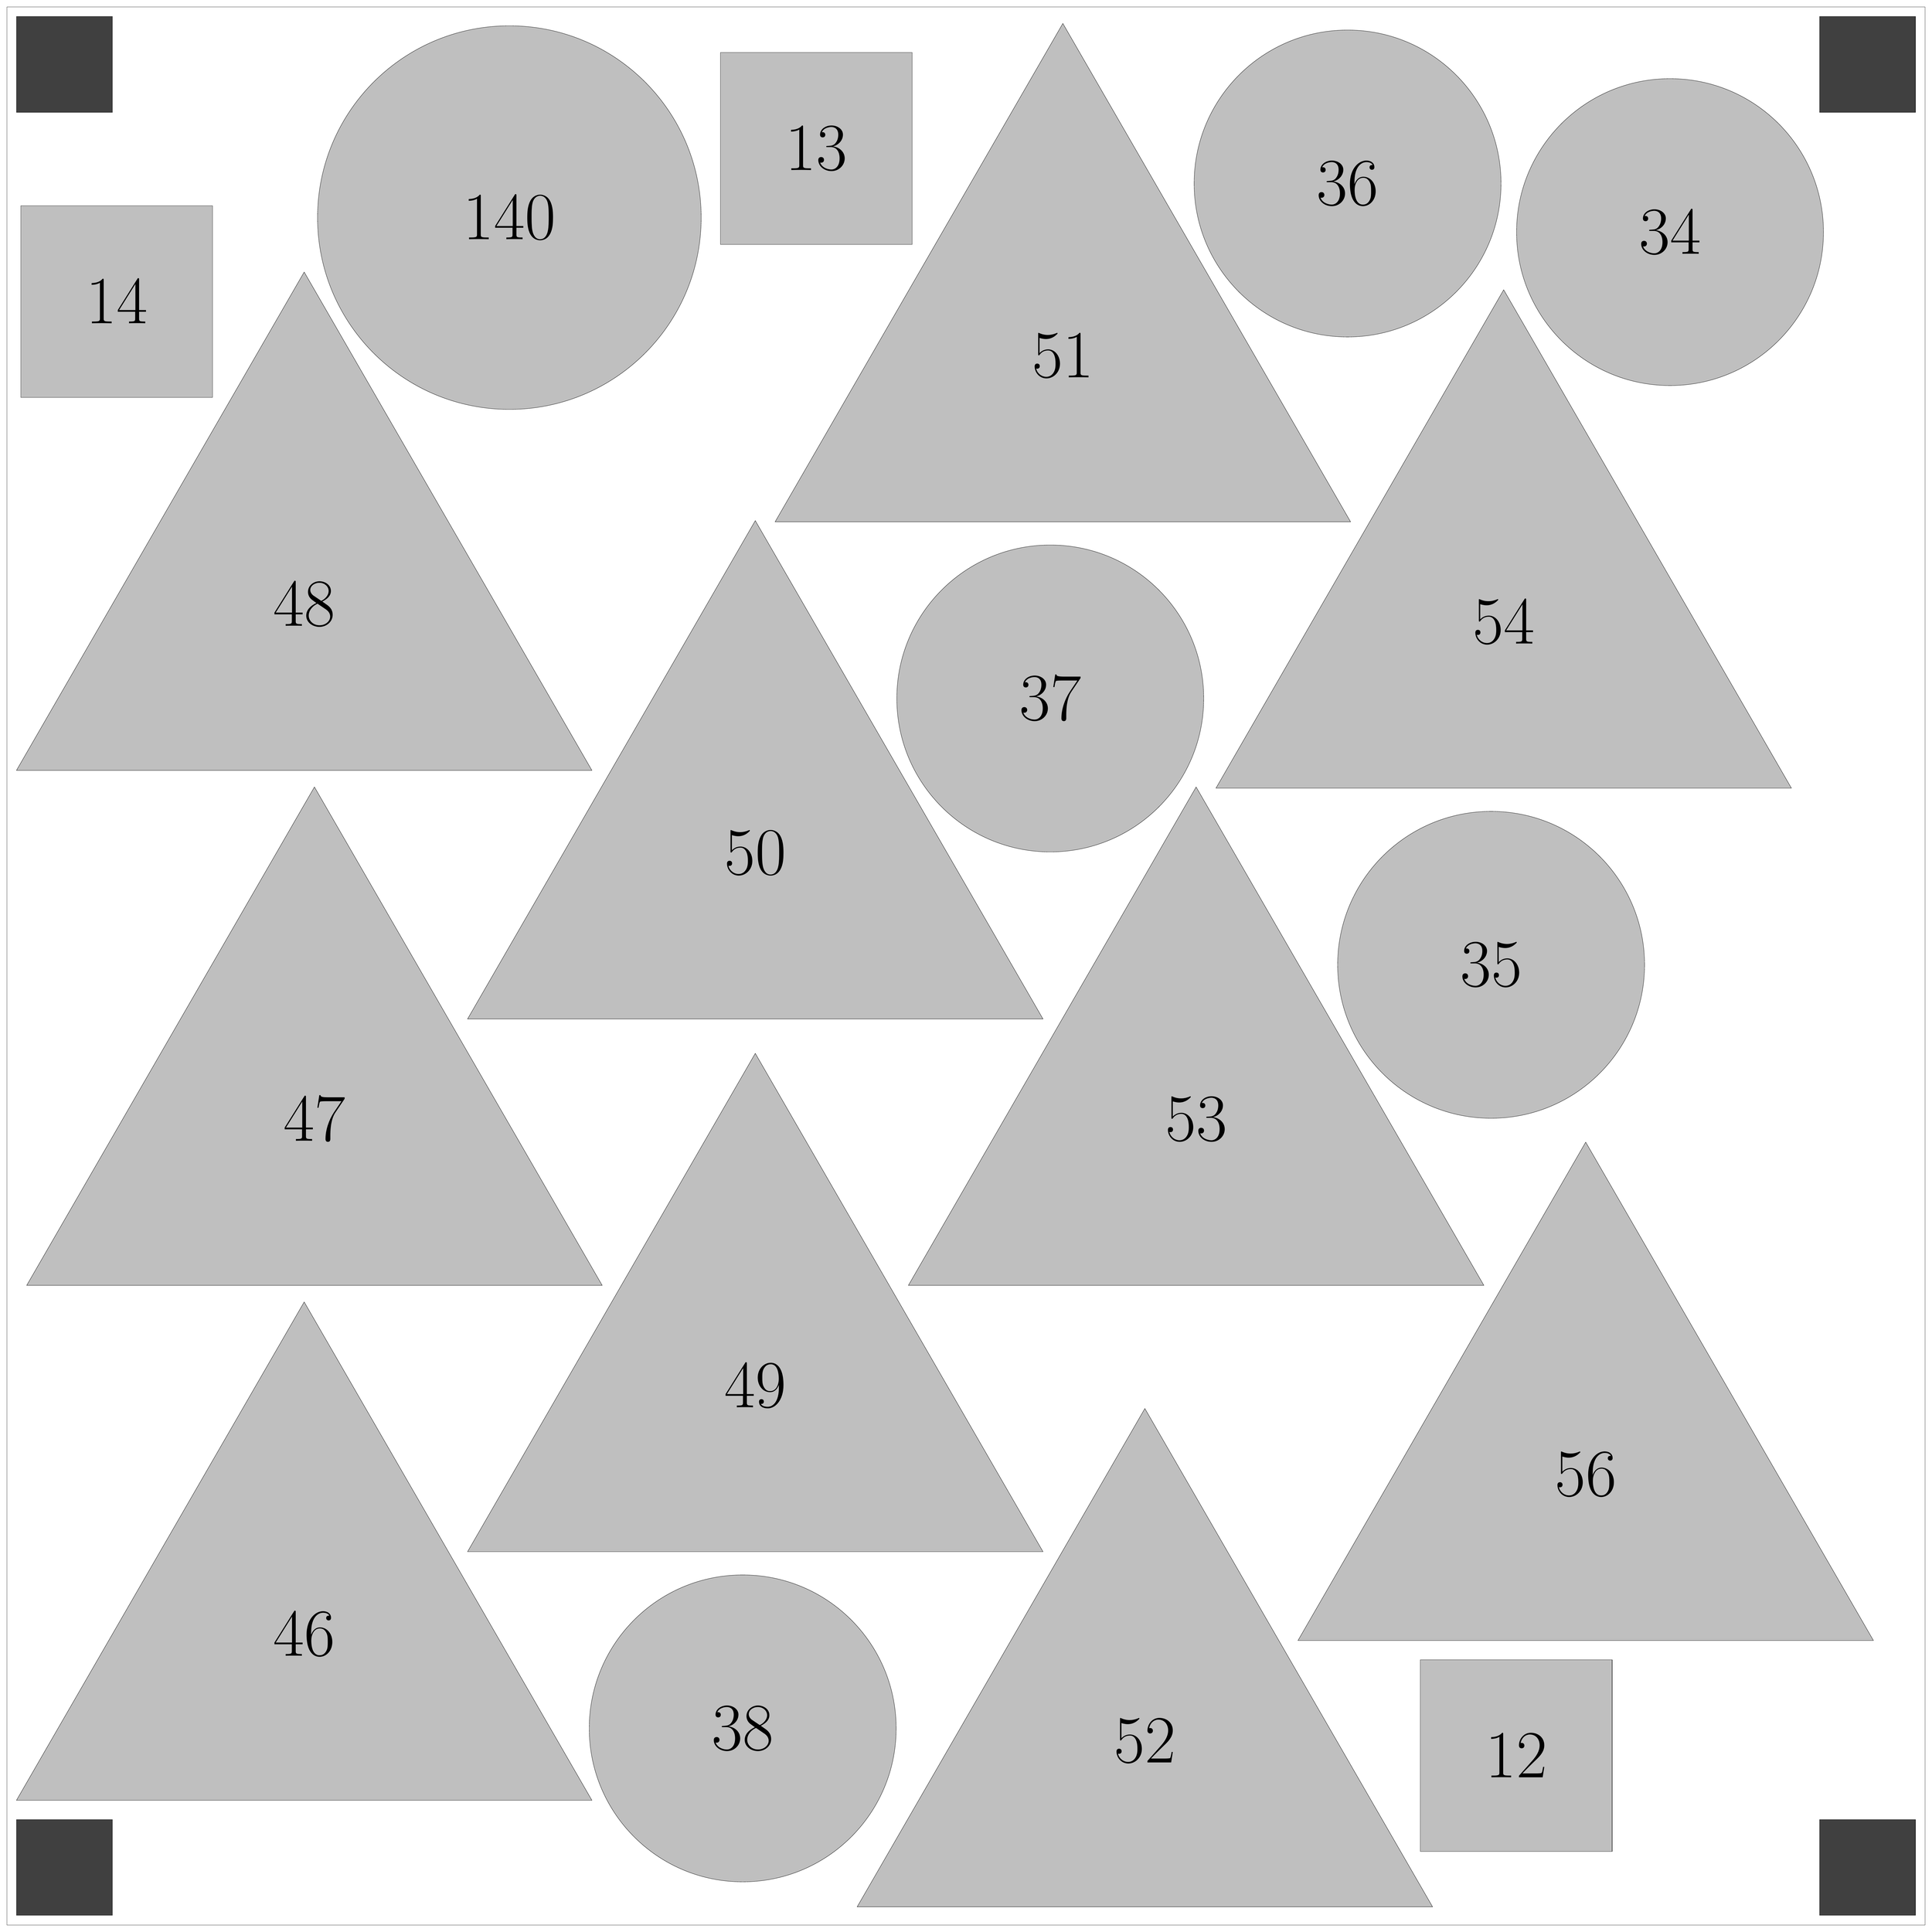
\begin{tikzpicture}\draw[black] (0,0) rectangle (100, 100);
\draw[black, fill=darkgray] (0.5,0.5) rectangle (5.5, 5.5);
\draw[black, fill=darkgray] (0.5,94.5) rectangle (5.5, 99.5);
\draw[black, fill=darkgray] (94.5,0.5) rectangle (99.5, 5.5);
\draw[black, fill=darkgray] (94.5,94.5) rectangle (99.5, 99.5);
\draw[black, fill=lightgray] (0.5,6.5) -- (30.5, 6.5) -- (15.5, 32.4808) -- cycle;
\draw (15.5, 15.1603) node {\fontsize{100}{120}\selectfont 46};
\draw[black, fill=lightgray] (1.03448,33.3468) -- (31.0345, 33.3468) -- (16.0345, 59.3275) -- cycle;
\draw (16.0345, 42.007) node {\fontsize{100}{120}\selectfont 47};
\draw[black, fill=lightgray] (0.5,60.1936) -- (30.5, 60.1936) -- (15.5, 86.1743) -- cycle;
\draw (15.5, 68.8538) node {\fontsize{100}{120}\selectfont 48};
\draw[black, fill=lightgray] (24.0172,19.4605) -- (54.0172, 19.4605) -- (39.0172, 45.4413) -- cycle;
\draw (39.0172, 28.1208) node {\fontsize{100}{120}\selectfont 49};
\draw[black, fill=lightgray] (24.0172,47.2331) -- (54.0172, 47.2331) -- (39.0172, 73.2138) -- cycle;
\draw (39.0172, 55.8933) node {\fontsize{100}{120}\selectfont 50};
\draw[black, fill=lightgray] (40.0517,73.1541) -- (70.0517, 73.1541) -- (55.0517, 99.1349) -- cycle;
\draw (55.0517, 81.8143) node {\fontsize{100}{120}\selectfont 51};
\draw[black, fill=lightgray] (44.3276,0.945492) -- (74.3276, 0.945492) -- (59.3276, 26.9263) -- cycle;
\draw (59.3276, 9.60575) node {\fontsize{100}{120}\selectfont 52};
\draw[black, fill=lightgray] (47,33.3468) -- (77, 33.3468) -- (62, 59.3275) -- cycle;
\draw (62, 42.007) node {\fontsize{100}{120}\selectfont 53};
\draw[black, fill=lightgray] (63.0345,59.2678) -- (93.0345, 59.2678) -- (78.0345, 85.2486) -- cycle;
\draw (78.0345, 67.9281) node {\fontsize{100}{120}\selectfont 54};
\draw[black, fill=lightgray] (67.3103,14.8318) -- (97.3103, 14.8318) -- (82.3103, 40.8125) -- cycle;
\draw (82.3103, 23.492) node {\fontsize{100}{120}\selectfont 56};
\draw[black, fill=lightgray] (26.1967,89.0131) circle (10);
\draw (26.1967, 89.0131) node {\fontsize{100}{120}\selectfont 140};
\draw[black, fill=lightgray] (38.3612,10.25) circle (8);
\draw (38.3612, 10.25) node {\fontsize{100}{120}\selectfont 38};
\draw[black, fill=lightgray] (54.3957,63.9436) circle (8);
\draw (54.3957, 63.9436) node {\fontsize{100}{120}\selectfont 37};
\draw[black, fill=lightgray] (69.8957,90.7904) circle (8);
\draw (69.8957, 90.7904) node {\fontsize{100}{120}\selectfont 36};
\draw[black, fill=lightgray] (77.3785,50.0573) circle (8);
\draw (77.3785, 50.0573) node {\fontsize{100}{120}\selectfont 35};
\draw[black, fill=lightgray] (86.7058,88.2566) circle (8);
\draw (86.7058, 88.2566) node {\fontsize{100}{120}\selectfont 34};
\draw[black, fill=lightgray] (0.724138,79.6344) rectangle (10.7241, 89.6344);
\draw (5.72414, 84.6344) node {\fontsize{100}{120}\selectfont 14};
\draw[black, fill=lightgray] (37.1967,87.6166) rectangle (47.1967, 97.6166);
\draw (42.1967, 92.6166) node {\fontsize{100}{120}\selectfont 13};
\draw[black, fill=lightgray] (73.6897,3.83176) rectangle (83.6897, 13.8318);
\draw (78.6897, 8.83176) node {\fontsize{100}{120}\selectfont 12};\end{tikzpicture}
}%
\newpage\clearpage
\thispagestyle{empty}
\begin{center} 
\large\textbf{9\degree Andar}\\
\vspace*{5px} 
\large
\textmd{Comprimento: 100  -  Profundidade: 100  -  Altura: 20 (cm)}\\ \end{center}
\centering
\resizebox{!}{0.9\textheight}{%
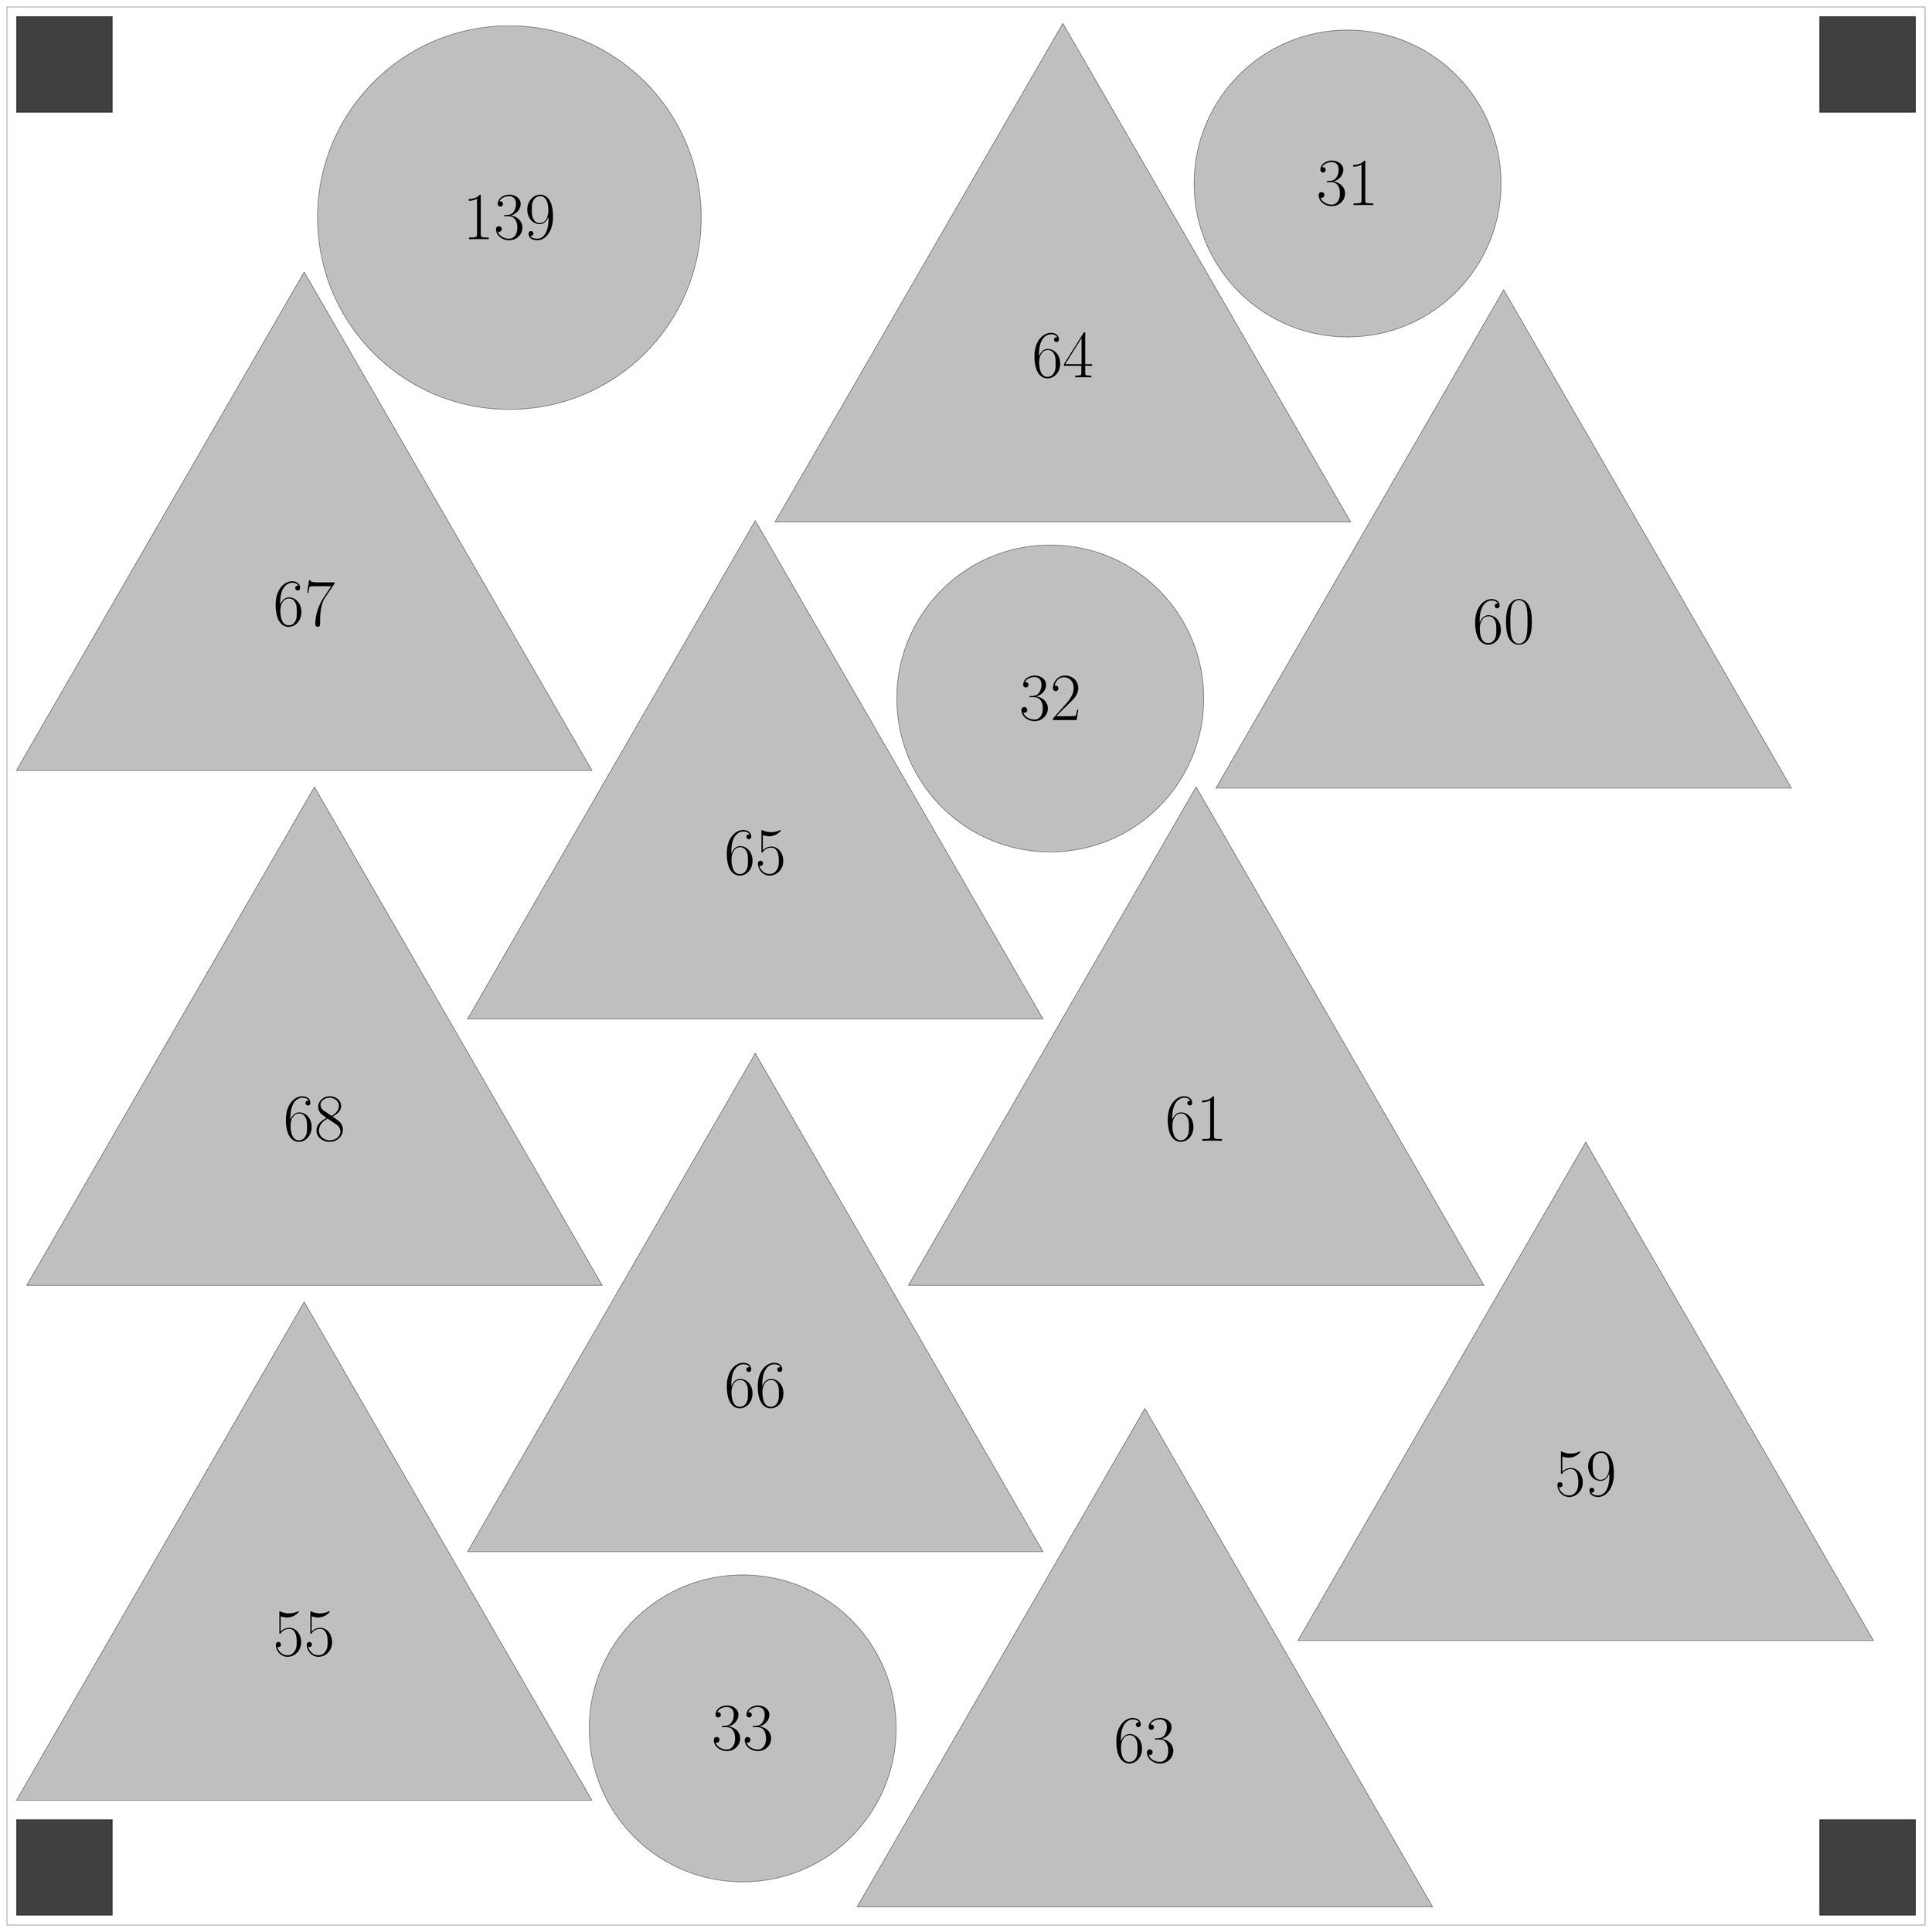
\begin{tikzpicture}\draw[black] (0,0) rectangle (100, 100);
\draw[black, fill=darkgray] (0.5,0.5) rectangle (5.5, 5.5);
\draw[black, fill=darkgray] (0.5,94.5) rectangle (5.5, 99.5);
\draw[black, fill=darkgray] (94.5,0.5) rectangle (99.5, 5.5);
\draw[black, fill=darkgray] (94.5,94.5) rectangle (99.5, 99.5);
\draw[black, fill=lightgray] (0.5,6.5) -- (30.5, 6.5) -- (15.5, 32.4808) -- cycle;
\draw (15.5, 15.1603) node {\fontsize{100}{120}\selectfont 55};
\draw[black, fill=lightgray] (1.03448,33.3468) -- (31.0345, 33.3468) -- (16.0345, 59.3275) -- cycle;
\draw (16.0345, 42.007) node {\fontsize{100}{120}\selectfont 68};
\draw[black, fill=lightgray] (0.5,60.1936) -- (30.5, 60.1936) -- (15.5, 86.1743) -- cycle;
\draw (15.5, 68.8538) node {\fontsize{100}{120}\selectfont 67};
\draw[black, fill=lightgray] (24.0172,19.4605) -- (54.0172, 19.4605) -- (39.0172, 45.4413) -- cycle;
\draw (39.0172, 28.1208) node {\fontsize{100}{120}\selectfont 66};
\draw[black, fill=lightgray] (24.0172,47.2331) -- (54.0172, 47.2331) -- (39.0172, 73.2138) -- cycle;
\draw (39.0172, 55.8933) node {\fontsize{100}{120}\selectfont 65};
\draw[black, fill=lightgray] (40.0517,73.1541) -- (70.0517, 73.1541) -- (55.0517, 99.1349) -- cycle;
\draw (55.0517, 81.8143) node {\fontsize{100}{120}\selectfont 64};
\draw[black, fill=lightgray] (44.3276,0.945492) -- (74.3276, 0.945492) -- (59.3276, 26.9263) -- cycle;
\draw (59.3276, 9.60575) node {\fontsize{100}{120}\selectfont 63};
\draw[black, fill=lightgray] (47,33.3468) -- (77, 33.3468) -- (62, 59.3275) -- cycle;
\draw (62, 42.007) node {\fontsize{100}{120}\selectfont 61};
\draw[black, fill=lightgray] (63.0345,59.2678) -- (93.0345, 59.2678) -- (78.0345, 85.2486) -- cycle;
\draw (78.0345, 67.9281) node {\fontsize{100}{120}\selectfont 60};
\draw[black, fill=lightgray] (67.3103,14.8318) -- (97.3103, 14.8318) -- (82.3103, 40.8125) -- cycle;
\draw (82.3103, 23.492) node {\fontsize{100}{120}\selectfont 59};
\draw[black, fill=lightgray] (26.1967,89.0131) circle (10);
\draw (26.1967, 89.0131) node {\fontsize{100}{120}\selectfont 139};
\draw[black, fill=lightgray] (38.3612,10.25) circle (8);
\draw (38.3612, 10.25) node {\fontsize{100}{120}\selectfont 33};
\draw[black, fill=lightgray] (54.3957,63.9436) circle (8);
\draw (54.3957, 63.9436) node {\fontsize{100}{120}\selectfont 32};
\draw[black, fill=lightgray] (69.8957,90.7904) circle (8);
\draw (69.8957, 90.7904) node {\fontsize{100}{120}\selectfont 31};\end{tikzpicture}
}%
\newpage\clearpage
\thispagestyle{empty}
\begin{center} 
\large\textbf{10\degree Andar}\\
\vspace*{5px} 
\large
\textmd{Comprimento: 100  -  Profundidade: 100  -  Altura: 20 (cm)}\\ \end{center}
\centering
\resizebox{!}{0.9\textheight}{%
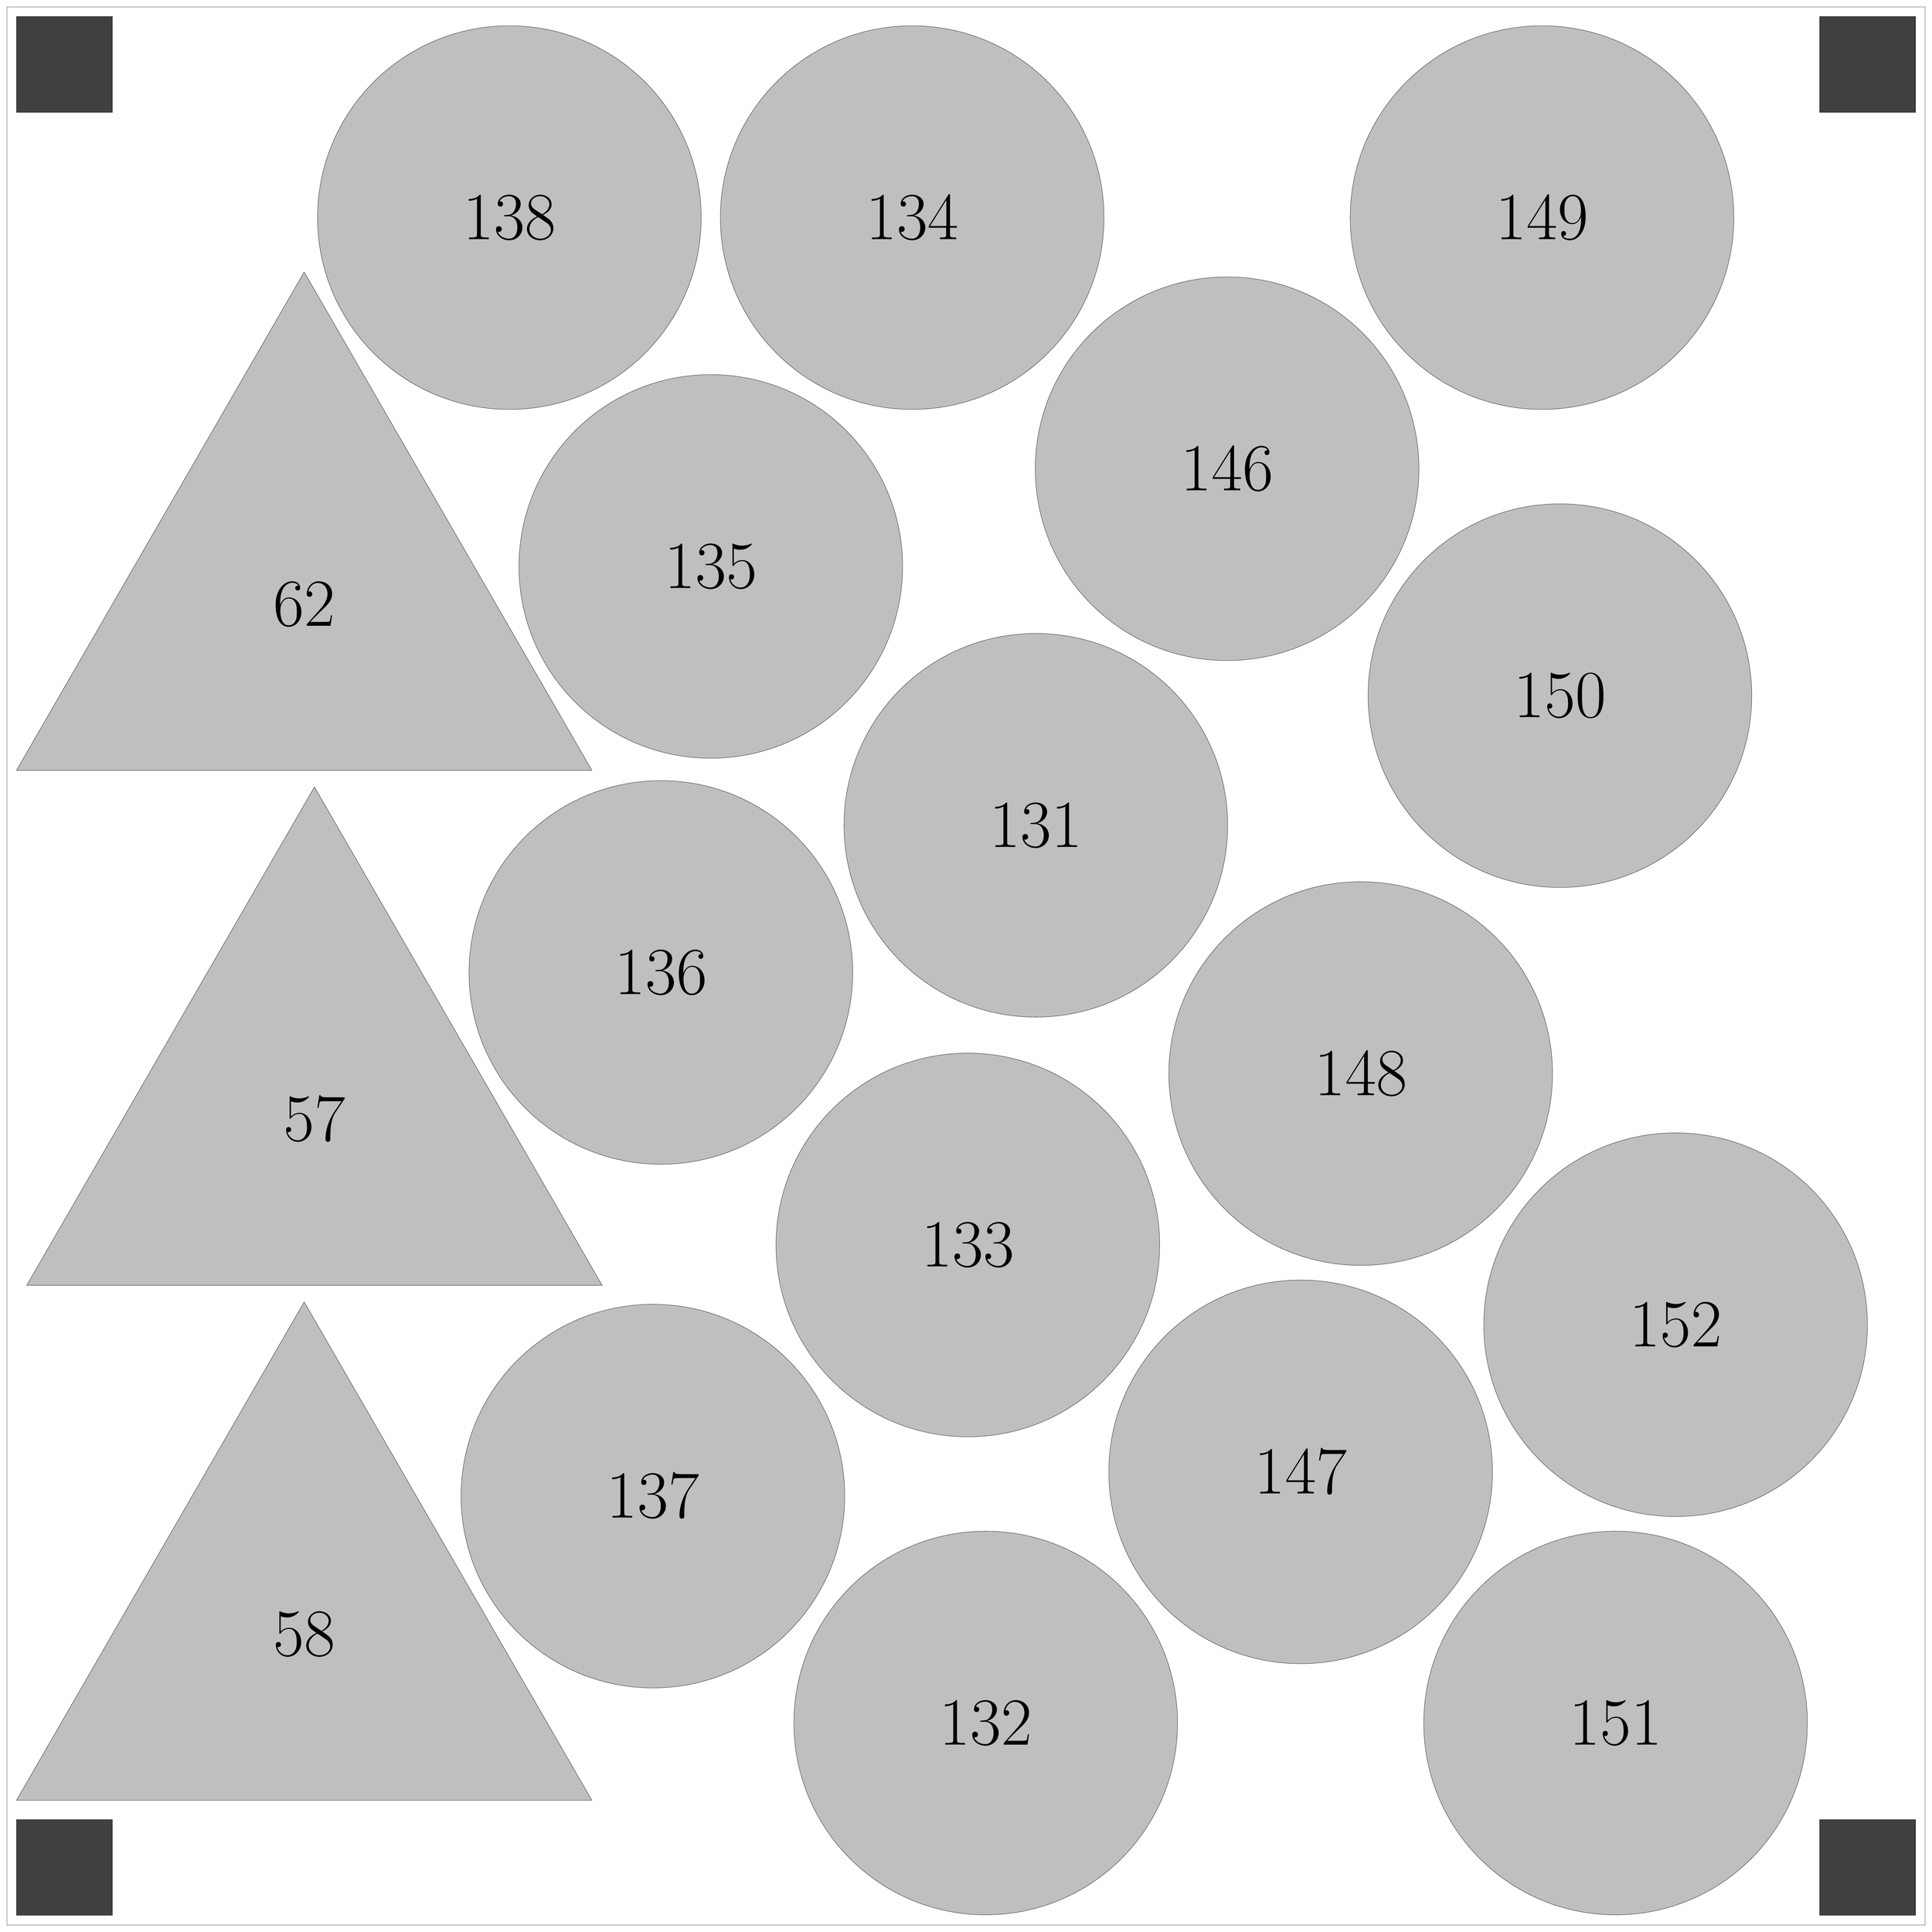
\begin{tikzpicture}\draw[black] (0,0) rectangle (100, 100);
\draw[black, fill=darkgray] (0.5,0.5) rectangle (5.5, 5.5);
\draw[black, fill=darkgray] (0.5,94.5) rectangle (5.5, 99.5);
\draw[black, fill=darkgray] (94.5,0.5) rectangle (99.5, 5.5);
\draw[black, fill=darkgray] (94.5,94.5) rectangle (99.5, 99.5);
\draw[black, fill=lightgray] (0.5,6.5) -- (30.5, 6.5) -- (15.5, 32.4808) -- cycle;
\draw (15.5, 15.1603) node {\fontsize{100}{120}\selectfont 58};
\draw[black, fill=lightgray] (1.03448,33.3468) -- (31.0345, 33.3468) -- (16.0345, 59.3275) -- cycle;
\draw (16.0345, 42.007) node {\fontsize{100}{120}\selectfont 57};
\draw[black, fill=lightgray] (0.5,60.1936) -- (30.5, 60.1936) -- (15.5, 86.1743) -- cycle;
\draw (15.5, 68.8538) node {\fontsize{100}{120}\selectfont 62};
\draw[black, fill=lightgray] (26.1967,89.0131) circle (10);
\draw (26.1967, 89.0131) node {\fontsize{100}{120}\selectfont 138};
\draw[black, fill=lightgray] (33.6795,22.359) circle (10);
\draw (33.6795, 22.359) node {\fontsize{100}{120}\selectfont 137};
\draw[black, fill=lightgray] (34.0949,49.6601) circle (10);
\draw (34.0949, 49.6601) node {\fontsize{100}{120}\selectfont 136};
\draw[black, fill=lightgray] (36.6967,70.8266) circle (10);
\draw (36.6967, 70.8266) node {\fontsize{100}{120}\selectfont 135};
\draw[black, fill=lightgray] (47.1967,89.0131) circle (10);
\draw (47.1967, 89.0131) node {\fontsize{100}{120}\selectfont 134};
\draw[black, fill=lightgray] (50.0979,35.4523) circle (10);
\draw (50.0979, 35.4523) node {\fontsize{100}{120}\selectfont 133};
\draw[black, fill=lightgray] (51.0305,10.5293) circle (10);
\draw (51.0305, 10.5293) node {\fontsize{100}{120}\selectfont 132};
\draw[black, fill=lightgray] (53.6433,57.3322) circle (10);
\draw (53.6433, 57.3322) node {\fontsize{100}{120}\selectfont 131};
\draw[black, fill=lightgray] (63.6152,75.9198) circle (10);
\draw (63.6152, 75.9198) node {\fontsize{100}{120}\selectfont 146};
\draw[black, fill=lightgray] (67.4489,23.6226) circle (10);
\draw (67.4489, 23.6226) node {\fontsize{100}{120}\selectfont 147};
\draw[black, fill=lightgray] (70.5788,44.388) circle (10);
\draw (70.5788, 44.388) node {\fontsize{100}{120}\selectfont 148};
\draw[black, fill=lightgray] (80.0336,89.0131) circle (10);
\draw (80.0336, 89.0131) node {\fontsize{100}{120}\selectfont 149};
\draw[black, fill=lightgray] (80.9662,64.0901) circle (10);
\draw (80.9662, 64.0901) node {\fontsize{100}{120}\selectfont 150};
\draw[black, fill=lightgray] (83.8674,10.5293) circle (10);
\draw (83.8674, 10.5293) node {\fontsize{100}{120}\selectfont 151};
\draw[black, fill=lightgray] (86.9973,31.2947) circle (10);
\draw (86.9973, 31.2947) node {\fontsize{100}{120}\selectfont 152};\end{tikzpicture}
}%
\newpage\clearpage
\thispagestyle{empty}
\begin{center} 
\large\textbf{11\degree Andar}\\
\vspace*{5px} 
\large
\textmd{Comprimento: 100  -  Profundidade: 100  -  Altura: 20 (cm)}\\ \end{center}
\centering
\resizebox{!}{0.9\textheight}{%
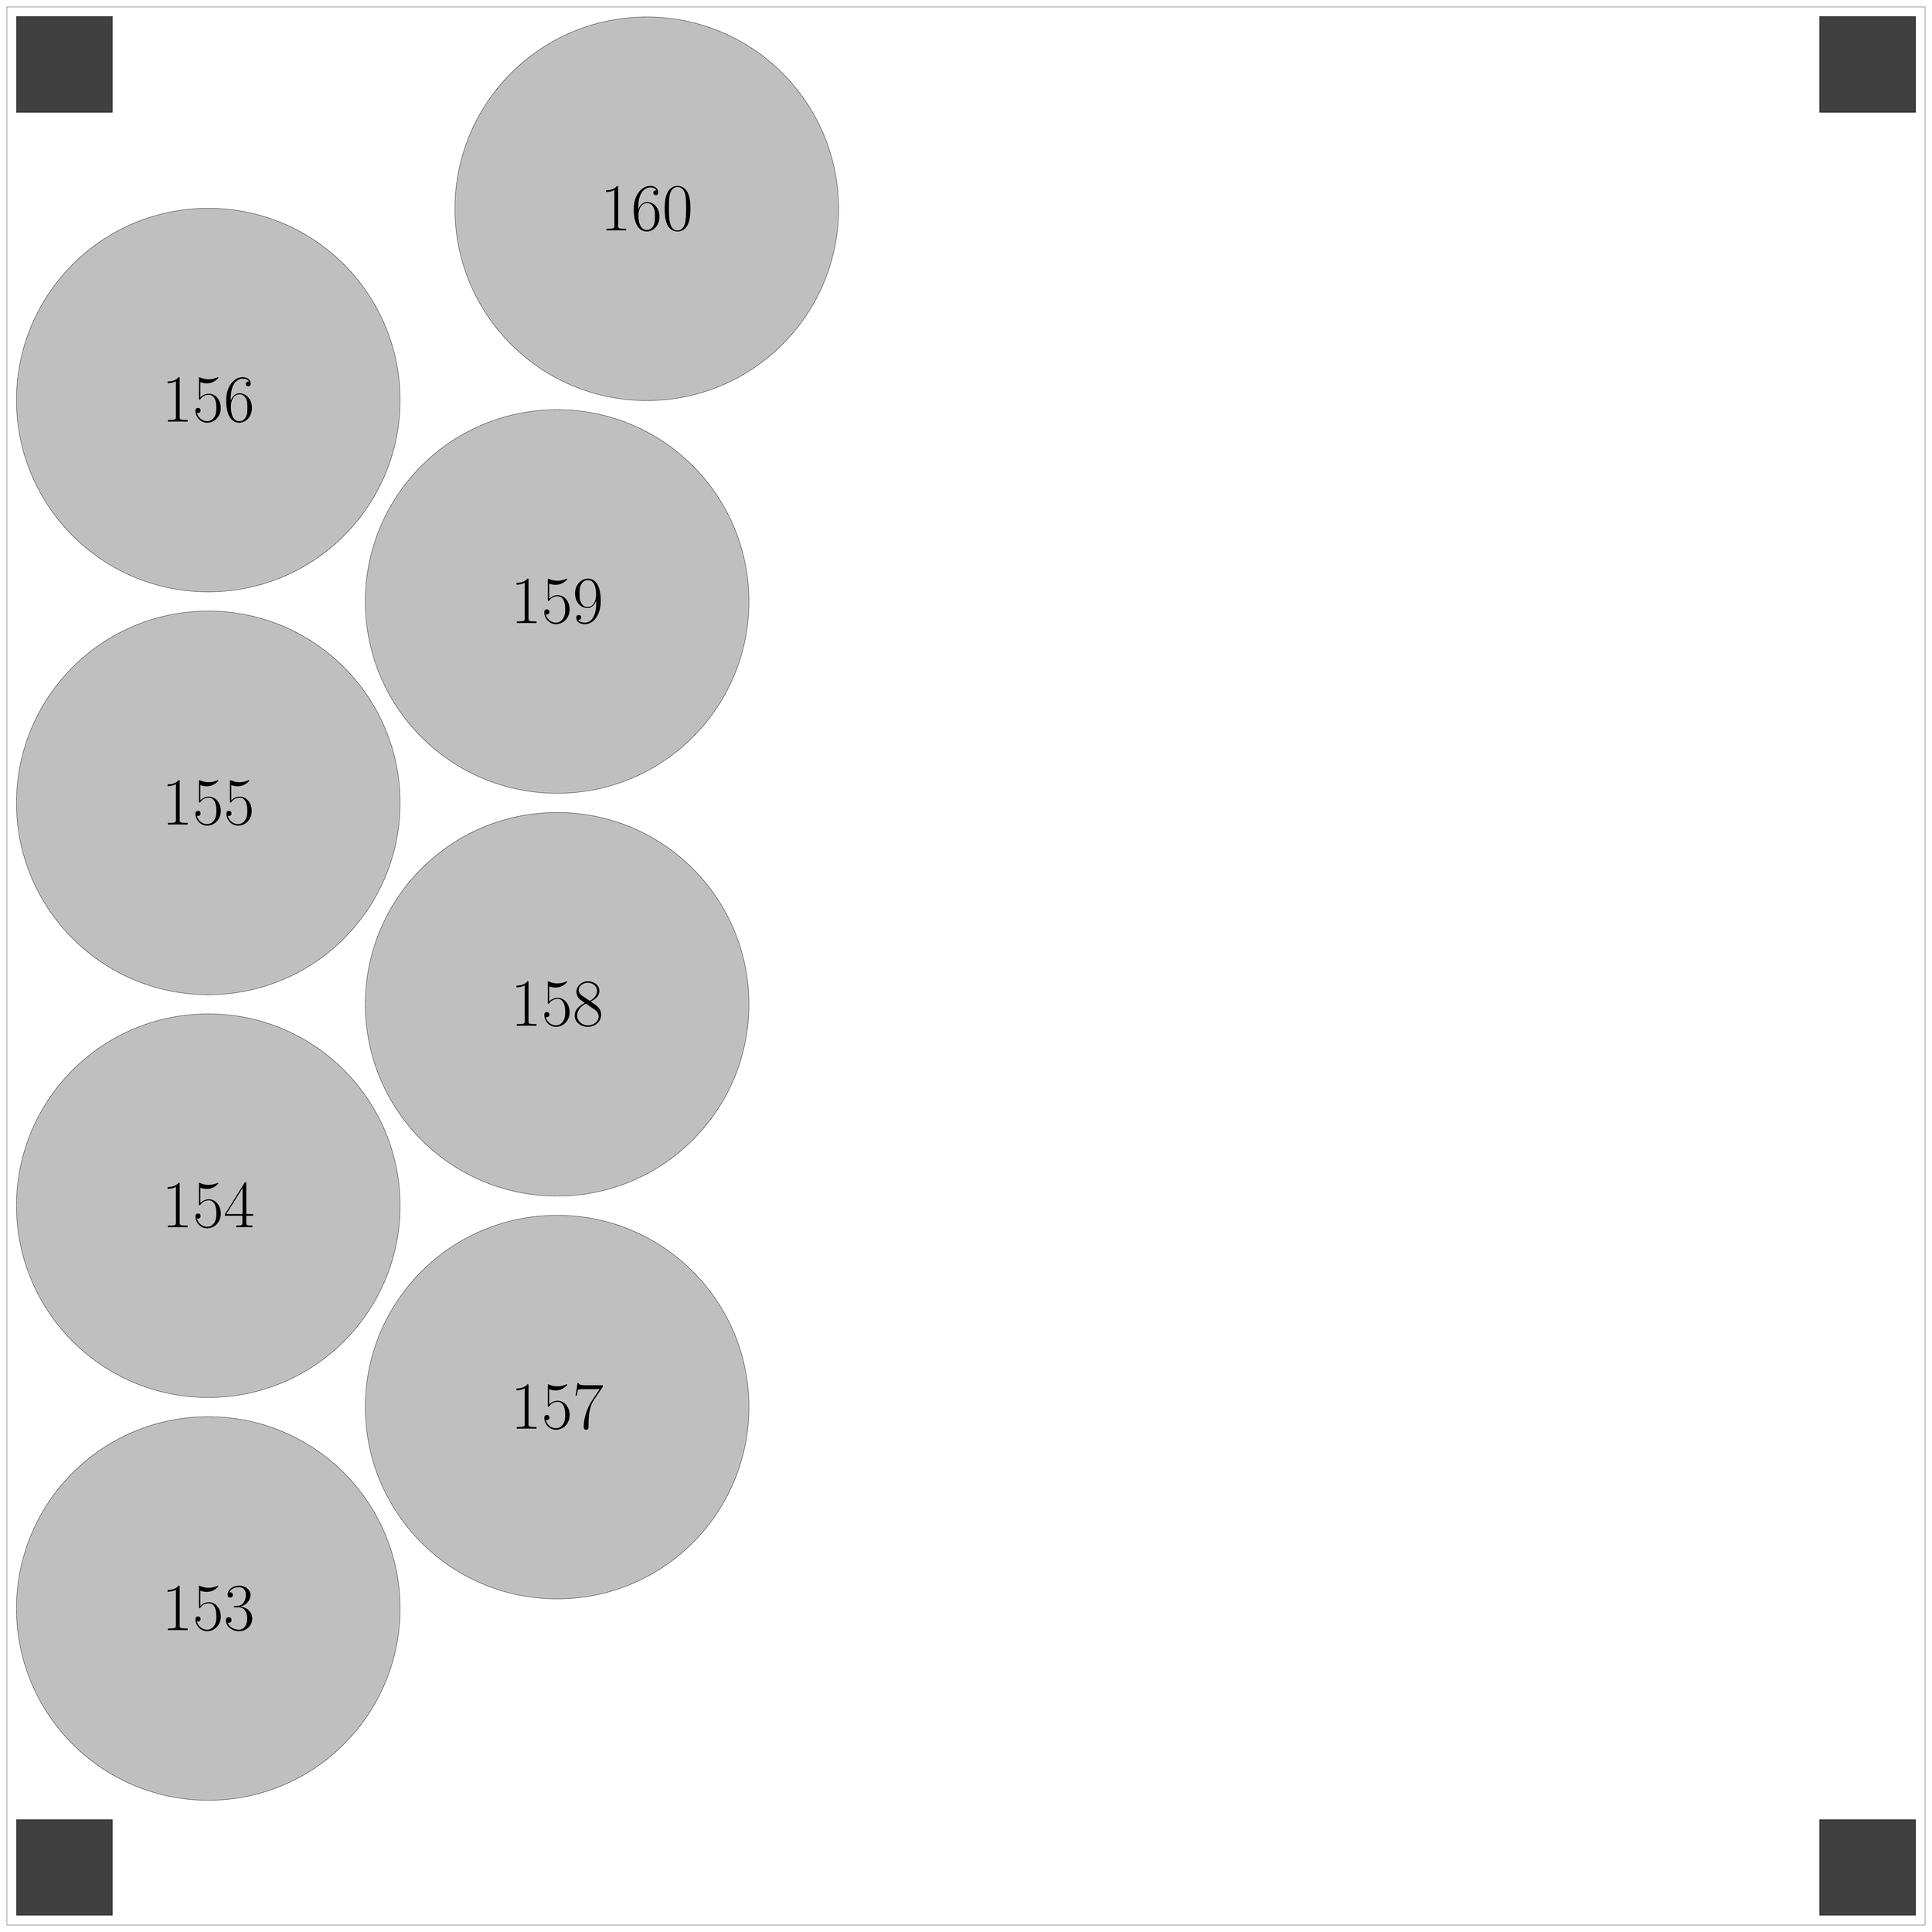
\begin{tikzpicture}\draw[black] (0,0) rectangle (100, 100);
\draw[black, fill=darkgray] (0.5,0.5) rectangle (5.5, 5.5);
\draw[black, fill=darkgray] (0.5,94.5) rectangle (5.5, 99.5);
\draw[black, fill=darkgray] (94.5,0.5) rectangle (99.5, 5.5);
\draw[black, fill=darkgray] (94.5,94.5) rectangle (99.5, 99.5);
\draw[black, fill=lightgray] (10.5,16.5) circle (10);
\draw (10.5, 16.5) node {\fontsize{100}{120}\selectfont 153};
\draw[black, fill=lightgray] (10.5,37.5) circle (10);
\draw (10.5, 37.5) node {\fontsize{100}{120}\selectfont 154};
\draw[black, fill=lightgray] (10.5,58.5) circle (10);
\draw (10.5, 58.5) node {\fontsize{100}{120}\selectfont 155};
\draw[black, fill=lightgray] (10.5,79.5) circle (10);
\draw (10.5, 79.5) node {\fontsize{100}{120}\selectfont 156};
\draw[black, fill=lightgray] (28.6865,27) circle (10);
\draw (28.6865, 27) node {\fontsize{100}{120}\selectfont 157};
\draw[black, fill=lightgray] (28.6865,48) circle (10);
\draw (28.6865, 48) node {\fontsize{100}{120}\selectfont 158};
\draw[black, fill=lightgray] (28.6865,69) circle (10);
\draw (28.6865, 69) node {\fontsize{100}{120}\selectfont 159};
\draw[black, fill=lightgray] (33.3595,89.4735) circle (10);
\draw (33.3595, 89.4735) node {\fontsize{100}{120}\selectfont 160};\end{tikzpicture}
}%
\newpage\clearpage\thispagestyle{empty}
\begin{center} 
\large
\textbf{Descrição das Peças}\\\vspace*{10px} 
 \end{center}\begin{enumerate}\item Testando_8
\item Testando_8
\item Testando_8
\item Testando_8
\item Testando_8
\item Testando_8
\item Testando_8
\item Testando_8
\item Testando_8
\item Testando_8
\item Testando_7
\item Testando_7
\item Testando_7
\item Testando_7
\item Testando_7
\item Testando_7
\item Testando_7
\item Testando_7
\item Testando_7
\item Testando_7
\item Testando_7
\item Testando_7
\item Testando_7
\item Testando_7
\item Testando_7
\item Testando_7
\item Testando_7
\item Testando_7
\item Testando_7
\item Testando_7
\item Testando_5
\item Testando_5
\item Testando_5
\item Testando_5
\item Testando_5
\item Testando_5
\item Testando_5
\item Testando_5
\item Testando_5
\item Testando_5
\item Testando_4
\item Testando_4
\item Testando_4
\item Testando_4
\item Testando_4
\item Testando_4
\item Testando_4
\item Testando_4
\item Testando_4
\item Testando_4
\item Testando_4
\item Testando_4
\item Testando_4
\item Testando_4
\item Testando_4
\item Testando_4
\item Testando_4
\item Testando_4
\item Testando_4
\item Testando_4
\item Testando_4
\item Testando_4
\item Testando_4
\item Testando_4
\item Testando_4
\item Testando_4
\item Testando_4
\item Testando_4
\item Testando_4
\item Testando_4
\item Testando_3
\item Testando_3
\item Testando_3
\item Testando_3
\item Testando_3
\item Testando_3
\item Testando_3
\item Testando_3
\item Testando_3
\item Testando_3
\item Testando_3
\item Testando_3
\item Testando_3
\item Testando_3
\item Testando_3
\item Testando_3
\item Testando_3
\item Testando_3
\item Testando_3
\item Testando_3
\item Testando_3
\item Testando_3
\item Testando_3
\item Testando_3
\item Testando_3
\item Testando_3
\item Testando_3
\item Testando_3
\item Testando_3
\item Testando_3
\item Testando_2
\item Testando_2
\item Testando_2
\item Testando_2
\item Testando_2
\item Testando_2
\item Testando_2
\item Testando_2
\item Testando_2
\item Testando_2
\item Testando_2
\item Testando_2
\item Testando_2
\item Testando_2
\item Testando_2
\item Testando_2
\item Testando_2
\item Testando_2
\item Testando_2
\item Testando_2
\item Testando_2
\item Testando_2
\item Testando_2
\item Testando_2
\item Testando_2
\item Testando_2
\item Testando_2
\item Testando_2
\item Testando_2
\item Testando_2
\item Testando_1
\item Testando_1
\item Testando_1
\item Testando_1
\item Testando_1
\item Testando_1
\item Testando_1
\item Testando_1
\item Testando_1
\item Testando_1
\item Testando_1
\item Testando_1
\item Testando_1
\item Testando_1
\item Testando_1
\item Testando_1
\item Testando_1
\item Testando_1
\item Testando_1
\item Testando_1
\item Testando_1
\item Testando_1
\item Testando_1
\item Testando_1
\item Testando_1
\item Testando_1
\item Testando_1
\item Testando_1
\item Testando_1
\item Testando_1
\end{enumerate}
\end{document}